\documentclass[preprint,12pt]{elsarticle}


%% The amssymb package provides various useful mathematical symbols
\usepackage{amssymb}
\usepackage{lineno,hyperref}
\usepackage{booktabs}
\usepackage{threeparttable}
\usepackage[capitalise]{cleveref}
\modulolinenumbers[1]

\journal{International Journal of Hydrogen Energy}
\bibliographystyle{elsarticle-num}

\begin{document}
	
	\begin{frontmatter}
		
		\title{Multi-objective optimization of ANN-based PSA model for hydrogen purification from steam-methane reforming gas}
		
		\author{Xiuxin Yu}
		\author{Yuanhui Shen}
		\author{Zhongbo Guan}
		\author{Donghui Zhang\corref{cor1}}
		\author{Zhongli Tang}
		\author{Wenbin Li}
		
		\cortext[cor1]{Corresponding author, E-mail address: donghuizhang@tju.edu.cn}
		\address{The Research Center of Chemical Engineering, School of Chemical Engineering and Technology, Tianjin University, Tianjin 300072, China}
		
		\begin{abstract}
			A 4-bed-8-step pressure swing adsorption (PSA) process has been developed to produce high-purity hydrogen from the steam methane reforming (SMR) gas mixture. The Detailed models have been established for hydrogen purification based on the experimentally determined parameters. Two surrogate models are investigated to optimize the process performance using artificial neural networks (ANN), which have been well trained by the samples, obtaining from the Detailed models using Latin hypercube sampling strategy. The results indicate that ANNs could approximate the performance and dynamic behavior of PSA process with extremely high accuracy. Herein, a robust and fast multi-objective optimization approach of PSA process using genetic algorithm on the basis of different ANN-based surrogate models has also been proposed, in which Dual- and Tri-objective optimizations are taken into account. This research shows that the method can not only find out the optimal operating conditions of the PSA process for hydrogen production with higher than 99\% accuracy, namely Pareto-Optimal Fronts, but also provide a reliable reference for operational enhancement.
		\end{abstract}
		
		%%Graphical abstract
		\begin{graphicalabstract}
			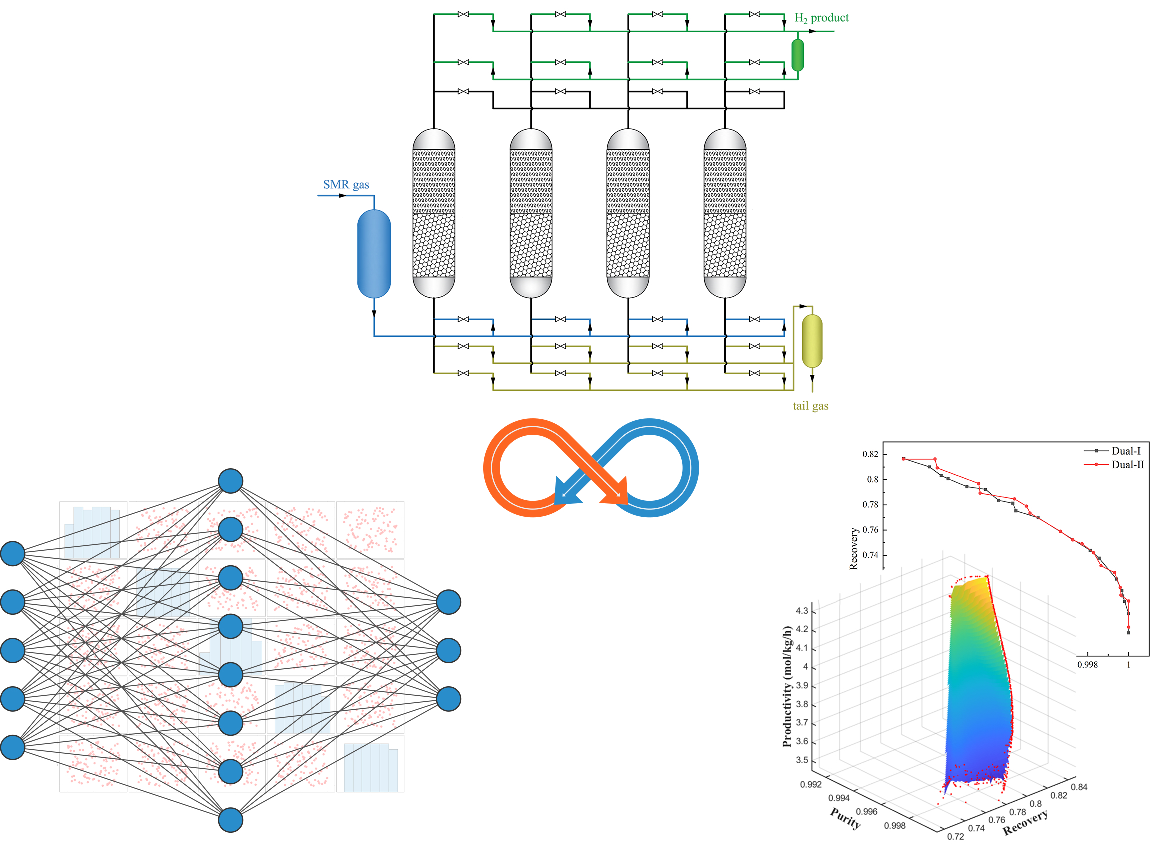
\includegraphics[width=1\textwidth]{figs/Graphical Abstract.pdf}
		\end{graphicalabstract}
		
		%%Research highlights
		\begin{highlights}
			\item Rigorous models for hydrogen production have been established
			\item Precise artificial neural networks were trained as surrogate models
			\item The Pareto-Optimal Fronts were achieved by multi-objective optimization with NSGA-\uppercase\expandafter{\romannumeral2}
		\end{highlights}
		
		\begin{keyword}
			Multiobjective optimization; Hydrogen production; Artificial Neural Network; Genetic algorithm; Pressure swing adsorption
		\end{keyword}
		
	\end{frontmatter}
	
	 \linenumbers
	
	%% main text
	\section{Introduction}
	Fossil fuels, such as coal, oil and natural gas, are the main energy source of human society, and this situation will even continue until 2050 \cite{RN1}. Due to the deterioration of global environmental caused by the utilization of fossil fuel \cite{RN2,RN3,RN4,RN5}, hydrogen, a clean and efficient energy, has been given bright expectations by researchers and considered as a crucial energy source in the future\cite{RN6,RN7,RN8,RN9}, which has been expected to contribute 90\% of energy consumption by 2080\cite{RN10}. Hydrogen is also a vital raw material in process industry, such as FT process\cite{RN11}, ammonia synthesis\cite{RN12} and petroleum industry\cite{RN13}. Various methods have been employed to produce hydrogen, including Hydrocarbon Reforming, Hydrocarbon Pyrolysis, Biomass Process and Water Splitting\cite{RN14}, and steam methane reforming (SMR) is currently the most cost-effective process\cite{RN15}. However, the product obtained from SMR is a gas mixture that includes hydrogen and other impurity gases. Pressure swing adsorption (PSA) is a highly mature and versatile gas separation and purification technology in the chemical industry\cite{RN16,RN17,RN18}, by which scholars and engineers have made a lot of efforts in the field of hydrogen production. Thus, there have been numerous developments and researches in this area reported recently\cite{RN8,RN19,RN20,RN21,RN22}. The purpose of this study was to try and establish a fast and reliable method to optimize the design of the PSA process and improve process performance.
	
	PSA is a typical dynamic process, and the detailed simulation must be achieved by solving a set of partial differential and algebraic equations (PDAEs)\cite{RN23,RN24}. However, owing to the gradually increasing complexity and scale of the simulation, engineers have encountered straits of process optimization, namely the huge time consumption of direct optimization on the system of PDAEs derives from many possible combinations of the design parameters\cite{RN25,RN26,RN27}. Sun et al. used detailed models to optimize a PSA process to recover CH4 from a gas mixture and the reduced space successive quadratic-programming (r-SQP) optimization algorithm is employed in the calculation, which took nearly 64 hours\cite{RN28}. Subraveti et al. solved the multi-objective optimization problem coupled with traditional optimization framework of detailed PSA models and it incurred significant computational costs, almost 4000 single-core hours\cite{RN29}. To avoid the large amount of time consumption required to reach the cyclic steady state (CSS) of PSA process, researchers have proposed a variety of different surrogate models to reduce the amount of calculation for the simulation and optimization, including response surface method, kriging models\cite{RN30,RN31,RN32}, proper orthogonal decomposition\cite{RN33}, polynomial regression (PNR) model\cite{RN19,RN25},  support vector regression\cite{RN25,RN34} and artificial neural network (ANN) model\cite{RN34,RN35}. All these models employ an input-output relationship based on observed dataset to predict the approximate performance of the process instead of solving the equation, but they can be divided into two types: \uppercase\expandafter{\romannumeral1}) explicit regression functions with fixed forms, such as, response surface method and polynomial regression model; \uppercase\expandafter{\romannumeral2}) implicit regression functions, such as support vector regression, ANN and more\cite{RN36}.
	
	To select the most suitable and precise model is crucial for data-driven optimization based on surrogate models. Artificial neural network is one of the most important tools used in machine learning, which is a brain-inspired system to replicate the way of humans learn. In recent decades, ANN has become a major part of artificial intelligence (AI) and widely been used in different fields, including image identification, autopilot, scenario prediction and so on. Industry 4.0 connects physics and digit with advanced technologies, such as the Internet of Things (IoT), Big data, AI and Machine learning, so it offers a more comprehensive, interlinked, and holistic approach to manufacturing\cite{RN37}. Recently, few literatures about ANN-based surrogate model of PSA process have been reported. Ma et al. established an ANN model to predict breakthrough curves which has rational accuracy and impressive speed for making prediction of performance\cite{RN38}. Subraveti et al. designed a surrogate model combined ANN and genetic algorithm to optimize a PSA process for precombustion CO2 capture, reducing calculation time by an order of magnitude\cite{RN29}. Nguyen et al. developed a dynamic-model-based ANN for the PSA units analyzed by singular value decomposition, and it was trained and tested within a marginal error less than 2\%\cite{RN35}. Anna et al. achieved the optimization of a PSA process for the separation of N2/CH4 based on a ANN surrogate model, and the optimization time decreased from 15.7h to 50s\cite{RN39}. Xiao et al. reported that ANN models were more predominant for optimizing PSA process than PNR model\cite{RN19}. According to the Universal Approximation Theorem, standard multilayer feedforward networks (FFN) can approximate any Borel measurable function with any desired degree of accuracy under one hidden layer and enough neurons\cite{RN40}. On balance, compared with other methods, the ANN model can predict the performance of the PSA process more accurately and quickly, and has excellent robustness and reliability under well training. Therefore, the ANNs are selected as surrogate models of the PSA hydrogen production process for multi-objective optimization in this study. 
	
	The systematic design and optimization of PSA process is a typical multi-objective optimization problem, which is composed of several objective functions that may be conflicting with another, and a set of equality and inequality constraints. Typically, the target process performances of PSA process for gas separation and purification include the purity and recovery of desirable product, as well as unit productivity and energy consumption. Instead of one optimal solution, multi-objective optimization leads to a string of optimal solutions called as Pareto-optimal solutions, because of the trade-off between all objectives. Various optimization methods are used by scholars to determine the decision variables of the PSA process and achieve the desired performance. The literature reported that gradient-based deterministic methods was recognized for the optimization of PSA\cite{RN33,RN41,RN42}, but these methods exist convergence problems while finding the global optimum point\cite{RN43}. Some methods can transform multi-objective optimization problems into single-objective optimization problems by constructing specific functions. Xiao et al. applied the linear weight sum method to combine purity with recovery and optimized the function using Interior Point optimization algorithm\cite{RN19,RN44}, and some researchers combine objective functions non-linearly to solve optimization problems\cite{RN11,RN34}. Pareto Evolutionary Techniques was suggested by Goldberg, taking advantage of non-dominated ranking and selection to solve multi-objective optimization problems\cite{RN45}. With the development of computer performance, some Pareto techniques have also been applied to optimize PSA process such as Non-dominated sorting genetic algorithm-\uppercase\expandafter{\romannumeral2} (NSGA-\uppercase\expandafter{\romannumeral2})\cite{RN29,RN32,RN34,RN46} and Multi-objective particle swarm optimization (MOPSO)\cite{RN11}, which have achieved excellent performance. The NSGA-\uppercase\expandafter{\romannumeral2} has been proven to have several advantages: \uppercase\expandafter{\romannumeral1}) it has excellent robustness for PSA process multi-objective optimization; \uppercase\expandafter{\romannumeral2}) it can avoid local minimums and provide Pareto optimal solutions; \uppercase\expandafter{\romannumeral3}) it could be parallelized easily on multi-core computers for reducing running time\cite{RN47}; \uppercase\expandafter{\romannumeral4}) it could be used to guide the design of experiment and process. In addition, the ANN-based surrogate models can meet the demands of a large population in the process of genetic algorithm optimization process without requiring enormous computational consumption. Therefore, the NSGA-\uppercase\expandafter{\romannumeral2} is selected to optimize the ANN-based surrogate models of the PSA unit for hydrogen production.
	
	In this work, a strategy of multi-objective optimization of ANN-based PSA surrogate models using genetic algorithm has been proposed to optimize the PSA process and improve process performance. A 4-bed-8-step PSA process to produce $H_2$ from SMR gas mixture was designed with activated carbon (AC) and zeolite 5A as adsorbents. Detailed PSA models have been built in Aspen Adsorption software based on experimentally measured isotherms and a set of PDAEs verified in our previous work. The machine learning models, two different ANNs, are well trained using the samples calculated from the detailed models based on the Latin Hypercube Sampling (LHS) strategy to fit the relations between decision variables and objective function of this PSA unit and forecast process performance, including purity, recovery and productivity. The Pareto-Optimal Fronts are obtained by multi-objective optimization using NSGA-\uppercase\expandafter{\romannumeral2} through different ANN-based surrogate models. The accuracy and reliability of these surrogate models and feasible solutions are discussed.
	\section{Experiments of equilibrium isotherms}
	The adsorption isotherms describe the saturated adsorption capacity ($q_i^*$) of the gas on the adsorbent at different pressures and temperatures, which is essential for accurately simulating the PSA process. The adsorption equilibria of pure $CH_4$, $CO_2$, CO and $H_2$ on the activated carbon and zeolite 5A were measured at 298.15K, 308.15K and 318.15K, respectively, using static volumetric method\cite{RN48,RN49}. The schematic diagram of the experimental apparatus is shown in the Supporting Information as Fig.S1 (S: Supporting Information; Same below). The multisite Extended Langmuir 2 equation\cite{RN50}, shown in  \cref{EXLang2}, is used to fit the isotherms in MATLAB Curve Fitting Toolbox. The Clausius-Clapeyron equation is used to calculate the isosteric heat of adsorption, given as \cref{CC}. The results of measurement experiments and fitted isotherms are displayed in Fig.1. Parameters $IP_{1,i}$,$IP_{2,i}$, $IP_{3,i}$ and $IP_{4,i}$ and values of heat of adsorption are demonstrated in Table S1.
	
	As illustrated in  \cref{FIG:1}, 5A has higher saturated adsorption capacity of CO than AC under low partial pressure of CO; CO2 is strongly adsorbed in 5A under extremely low partial pressure but poorly desorbed, however, the adsorption capacity of CO2 on AC is close to 5A and the isotherms are more linear, so it could be easier to regenerate. Thus, the layered bed was packed with AC and 5A at the bottom and top, respectively. AC is applied at the entrance of beds to avoid CO2 reach the next layer, 5A, that is used for deep purification to produce high purity H2.
	\begin{equation}
		q_i^* = \frac{{I{P_{1,i}} \cdot {e^{\frac{{I{P_{2,i}}}}{T}}} \cdot {P_i}}}{{1 + \sum\limits_{i = 1}^n I {P_{3,i}} \cdot {e^{\frac{{I{P_{4,i}}}}{T}}} \cdot {P_i}}}\label{EXLang2}
	\end{equation}	 
	 \begin{equation}
	 	\frac{{\Delta H}}{{R{T^2}}} =  - {\left( {\frac{{\partial \ln P}}{{\partial T}}} \right)_{\rm{q}}}\label{CC}
	 \end{equation}
	\begin{figure}
		\centering
		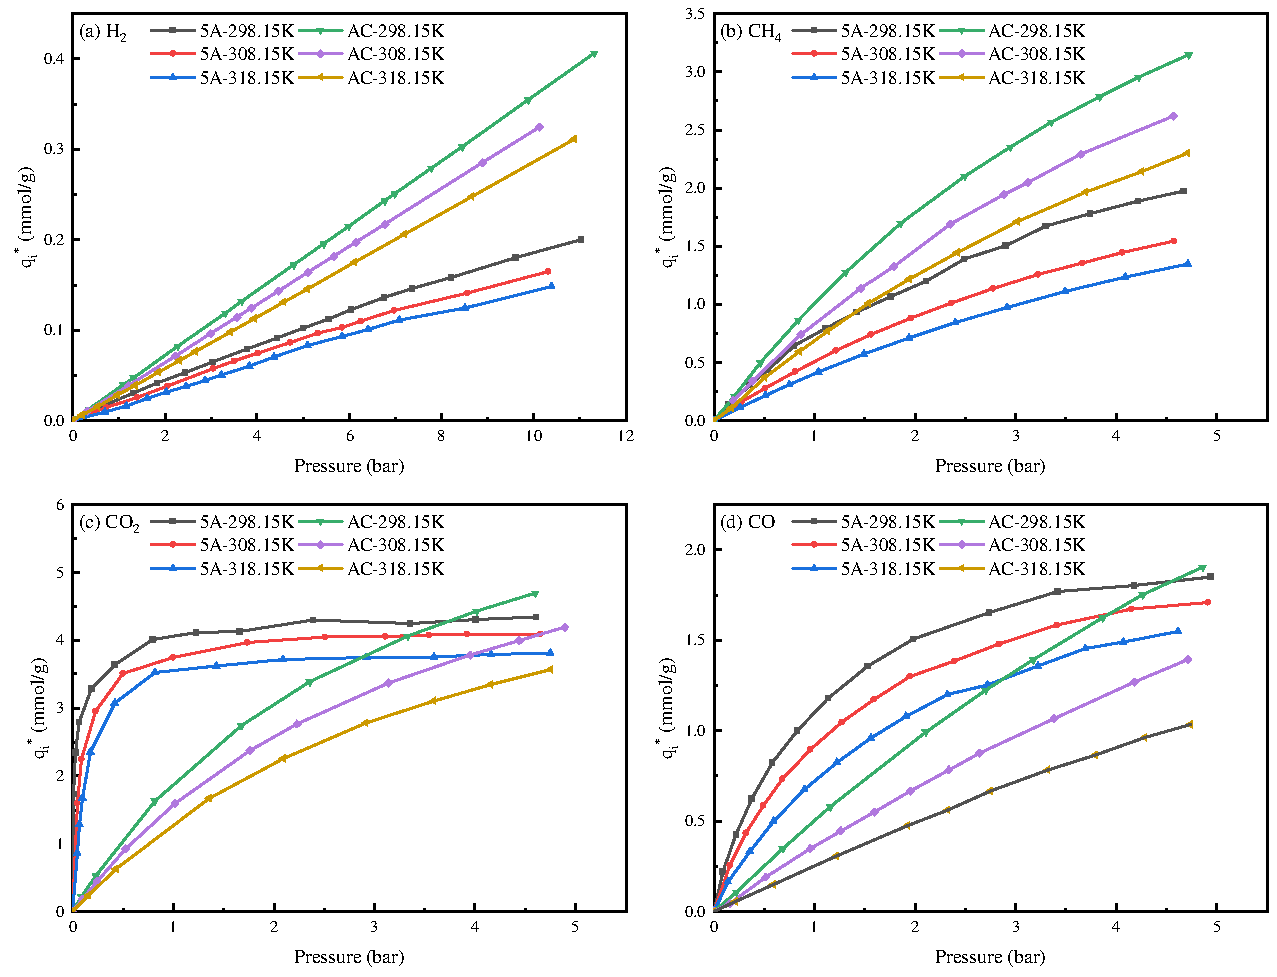
\includegraphics[width=1\textwidth]{figs/Fig1.pdf}
		\caption{Adsorption isotherm of H2(a), CH4(b), CO2(c) and CO(d) on zeolite 5A and AC}
		\label{FIG:1}
	\end{figure}
	\section{Detailed Model of PSA process}
	\subsection{Mathematical model}
	Pressure swing adsorption is a typical dynamic process, all variables change with time and space in cycles until the process achieves a cyclic steady state. The detailed simulations of PSA are achieved by solving a set of PDAEs, including mass transfer, heat transfer, momentum transfer and others. As the detailed mathematical model utilized in this work, it has been verified in our previous studies, enumerated in Supporting Information as Table S2, including numerical models of adsorption bed and auxiliary equipments. The boundary conditions associated with each step are given in Table S3. Moreover, the first-order upwind difference scheme (UDS1) is employed to discretize the mathematical model of adsorbent bed in axial, which transform PDAEs into time-related differential algebraic equations (DAEs), and the implicit Euler method was applied to solve the DAEs. The MA48 and Mixed Newton have been utilized for linear and nonlinear algebraic equations, respectively. Some reasonable assumptions are set to reduce the complexity of the system and accelerate the calculation:
	\begin{enumerate}
		\itemsep=0pt
		\item The gas phase is considered as an ideal gas.
		\item There is no radial variation in the gas concentration, temperature, and pressure.
		\item The pressure drop in adsorption bed is conformed to the Eugen equation.
		\item The bulk flow and adsorbents are in thermal equilibrium. 
		\item A linear driving force (LDF) model is used to describe the inter-phase mass transfer resistances.
		\item Porosity of beds and adsorbent particle is uniform along the adsorption bed.
	\end{enumerate}  
	Purity, Recovery and Productivity represent the performance of the PSA process and are also the objective function of optimization, calculated by the equations below:
	\begin{equation}
		Purity = \frac{{\int_0^{{t_{cycle}}} {{F_{out}}{y_{out,}}_{target}} dt}}{{\int_0^{{t_{cycle}}} {{F_{out}}dt} }}\label{Purity}
	\end{equation}
	\begin{equation}
		Recovery = \frac{{\int_0^{{t_{cycle}}} {{F_{out}}{y_{out,}}_{target}} dt}}{{\int_0^{{t_{cycle}}} {{F_{in}}{y_{in,target}}dt} }}\label{Recovery}
	\end{equation}
	\begin{equation}
		Productivity = 3600\frac{{\int_0^{{t_{cycle}}} {{F_{out}}{y_{out,product}}dt} }}{{{t_{cycle}}{m_{adsorbents}}}}   {\rm{(mol/kg/h)}}\label{Productivity}
	\end{equation}
	\subsection{Process description}
	A 4-bed-8-step PSA process is proposed with pressure equalization steps twice for producing high purity H2 from SMR gas, which contains 76\% H2, 20\% CO2, 3.5\% CH4 and 0.5\% CO. The layered-beds are applied in this unit, filling with activated carbon and zeolite 5A.The detailed model established in Aspen Adsorption with rigorous multi-bed approach is shown as \cref{FIG:2}. The parameters of the adsorbent bed and adsorbents are listed in \cref{TABLE:1} and \cref{TABLE:2}. The diagram of multi-bed model in Aspen Adsorption has been displayed in Fig.S2.
	\begin{figure}
		\centering
		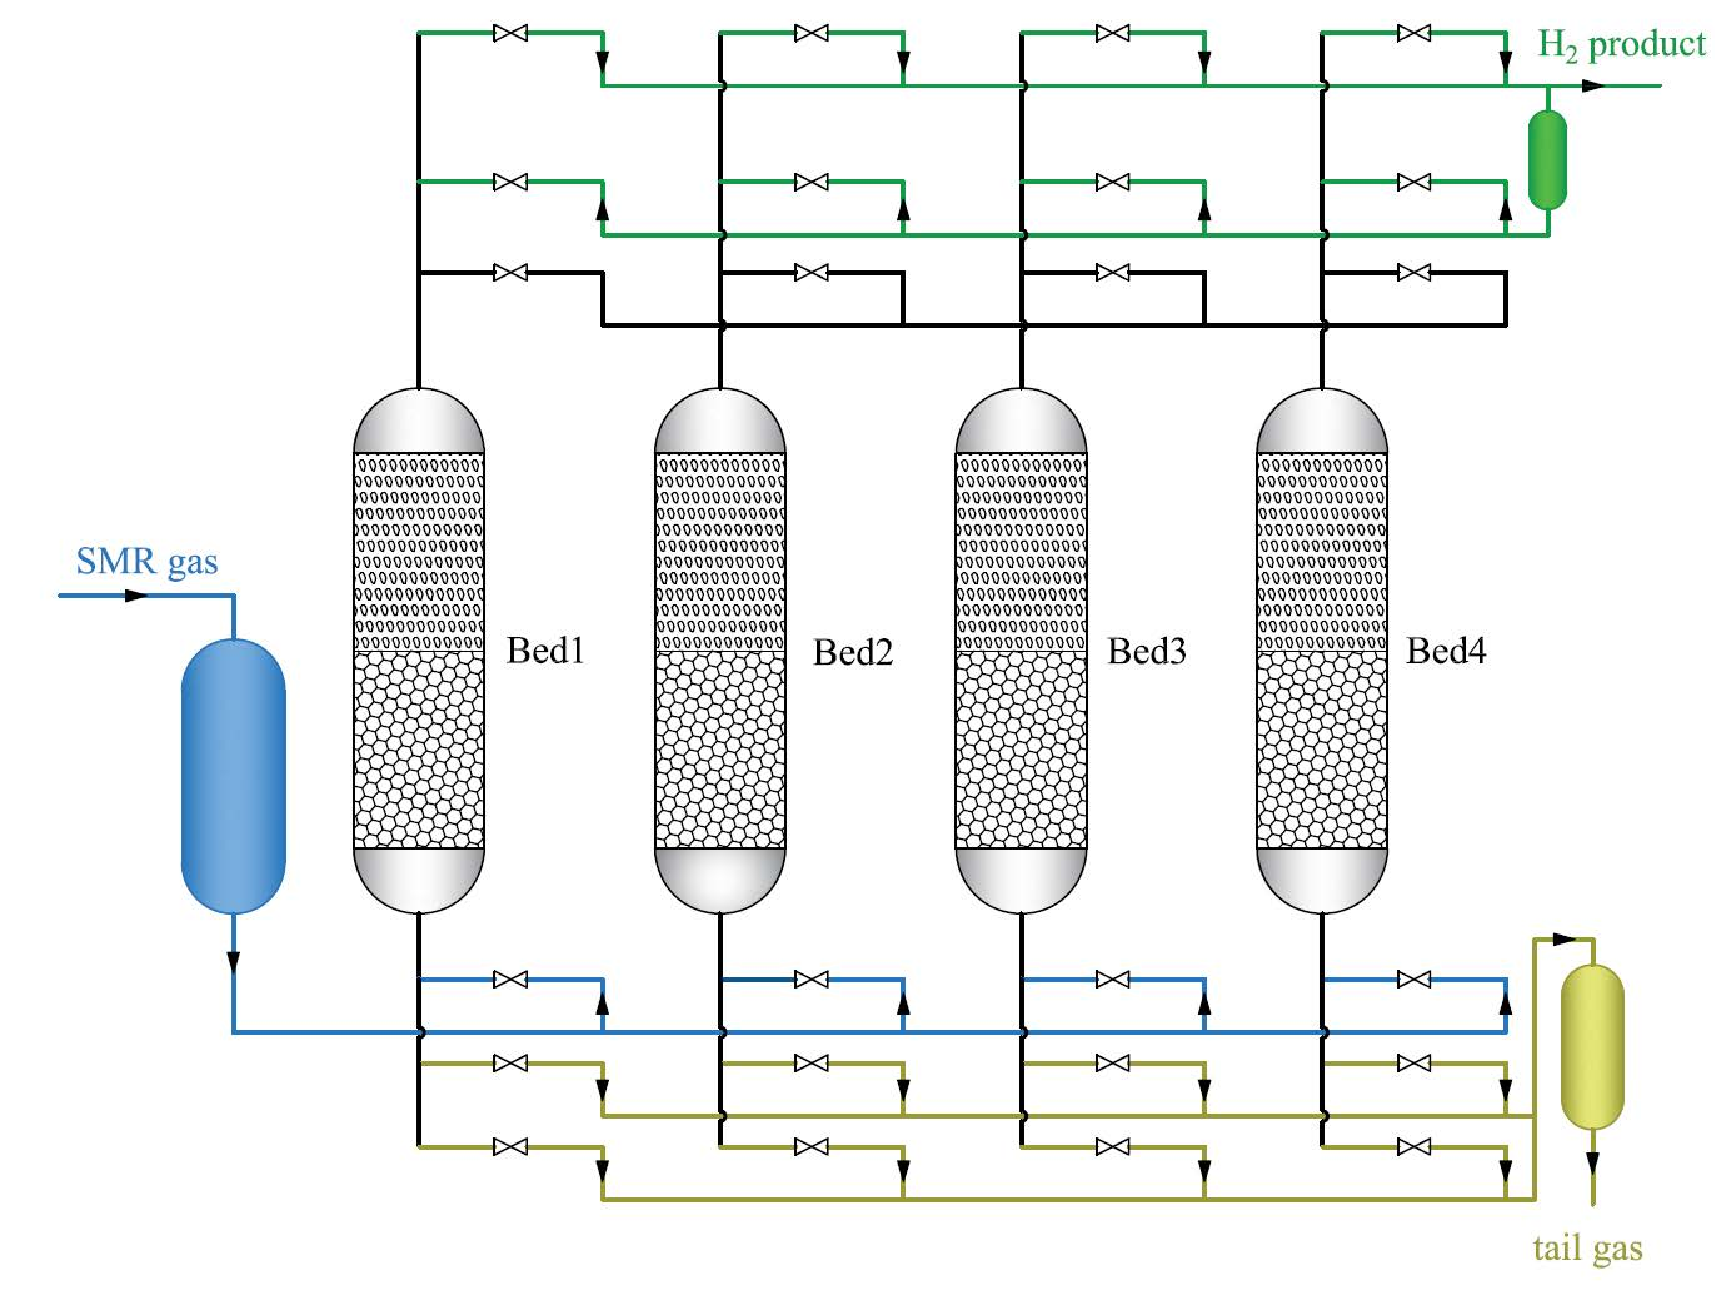
\includegraphics[width=1\textwidth]{figs/Fig2.pdf}
		\caption{Diagram of detailed model}
		\label{FIG:2}
	\end{figure}
\begin{table}[]
	\centering
	\caption{Parameters of beds and feed gas}
	\begin{tabular}{lll}
	\toprule
		Project                  & Value                                 &  \\
		\midrule
		Adsorption bed           &                                       &  \\
		Hb (m)                   & 1                                     &  \\
		Db (m)                   & 0.2                                   &  \\
		Bed number               & 4                                     &  \\
		Wb (m)                   & 0.02                                  &  \\
		Cpw (kJ·kg-1·K-1)        & 0.502                                 &  \\
		hw (W·m-2·K-1)           & 94                                    &  \\
		$\rho_w$ (kg·m-3)              & 7930                                  &  \\
		Feed gas                 &                                       &  \\
		Feed molar fraction (\%) & H2/CO2/CH4/CO = 0.76/0.20/0.035/0.005 &  \\
		hamb (W·m-2·K-1)         & 60                                    &  \\
		hf (W·m-2·K-1)           & 219                                   &  \\
		$\mu$ (Pa·s)                 & 1.75 E-5                              &  \\
		kg (W·m-2·K-1)           & 0.163                                 &  \\
		ks (W·m-2·K-1)           & 0.3                                   &  \\
		Tf (K)                   & 298.15                                &  \\
		$\eta_p$                       & 0.72                                  &  \\
		$\gamma$                        & 1.5                                   & \\
		\bottomrule
	\end{tabular}
	\label{TABLE:1}
\end{table}

\begin{table}[]
	\centering
	\caption{Parameters of the adsorbents}
	\begin{tabular}{lll}
		\toprule
		Project           & \multicolumn{2}{l}{Value}     \\
		\midrule
		Adsorbents        & 5A zeolite & Activated carbon \\
		$\epsilon_b$                & 0.357      & 0.35             \\
		$\epsilon_p$                 & 0.65       & 0.33             \\
		$\rho_b$  (kg·m-3)       & 698        & 522              \\
		rp (m)            & 1.6E-3     & 1.2E-3           \\
		Cps (kJ·kg-1·K-1) & 0.92       & 1.047        \\
		\bottomrule   
	\end{tabular}
	\label{TABLE:2}
\end{table}

\begin{figure}
	\centering
	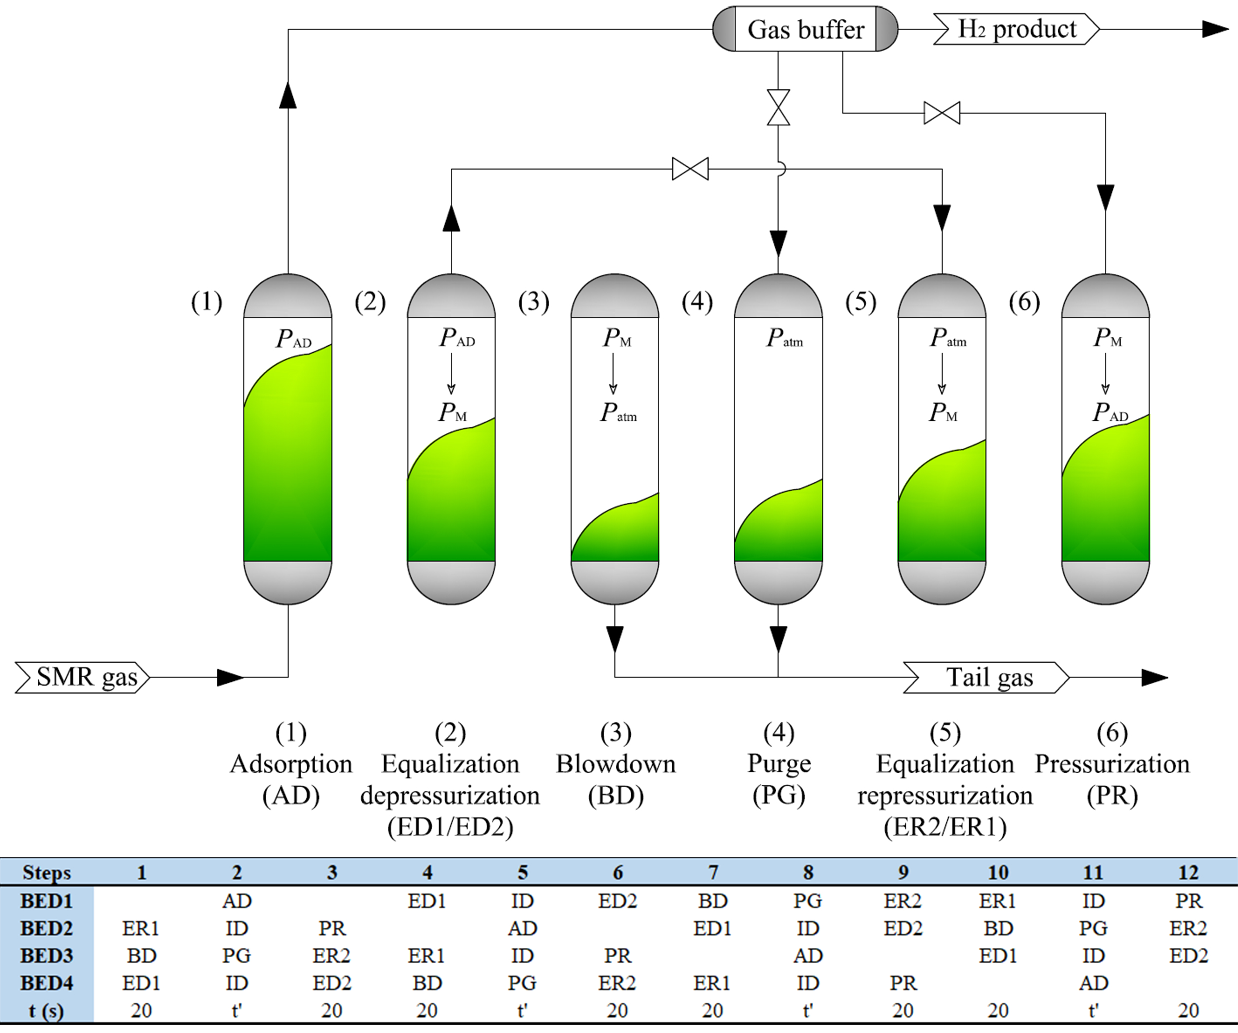
\includegraphics[width=1\textwidth]{figs/Fig3.pdf}
	\caption{Cycle sequence of PSA process}
	\label{FIG:3}
\end{figure}
The process takes 4*(20*2+t')s in one cycle, in which t' is one of the decision variables to be optimized. The cyclic sequences and detailed schematic diagram of each step are demonstrated in \cref{FIG:3}.

Step 1. Adsorption (AD). Feed gas, SMR mixture gas, enters from the bottom of the bed and high purity hydrogen with trace impurities exits in the bed, while heavy components are adsorbed at adsorbents.

Step 2. Equalization depressurization (ED1/ED2). PSA process with multiple pressure equalization steps could obtain higher H2 recovery. The gas flows from the high-pressure bed to the low-pressure bed driven by the pressure difference until the pressure is equalized.

Step 3. Blowdown (BD). The bed pressure drops to close to atmospheric pressure (Patm) due to the countercurrent discharge of gas.

Step 4. Purge (PG). The bed is purged by H2 product gas to regenerate the adsorbents.

Step 5. Equalization repressurization (ER2/ER1). The low-pressure bed receives gas from ED bed.

Step 6. Pressurization (PR). The hydrogen product reflux to bed to raise the pressure to adsorption pressure (PAD).

\section{Strategy and results of sampling}
\begin{table}[]
	\centering
	\caption{Boundaries of inputs variables}
	\begin{threeparttable}
	\begin{tabular}{llllll}
		\toprule
		& \begin{tabular}[c]{@{}l@{}}PAD\\    \\ (bar)\end{tabular} & \begin{tabular}[c]{@{}l@{}}t'\\    \\ (s)\end{tabular} & \begin{tabular}[c]{@{}l@{}}FAD\\    \\ (SLPM)\end{tabular} & \begin{tabular}[c]{@{}l@{}}LAC\\    \\ (m)\end{tabular} & \begin{tabular}[c]{@{}l@{}}P/F\\    \\ (-)\end{tabular} \\
		\midrule
		Lower boundary & 7                                                         & 100                                                    & 150                                                        & 0.3                                                     & 0.1                                                     \\
		Upper boundary & 9                                                         & 200                                                    & 200                                                        & 0.7                                                     & 0.2              \\
		\bottomrule                                      
	\end{tabular}
	\begin{tablenotes}
	\footnotesize
	\item {PAD: Pressure of adsorption; t': Part of adsorption time (40+ t'); FAD: Feed flowrate; LAC: Length of activated carbon layer (total length: 1m); P/F: Ratio of purge to feed.}
	\end{tablenotes}
\end{threeparttable}
	\label{TABLE:3}
\end{table}

\begin{figure}
	\centering
	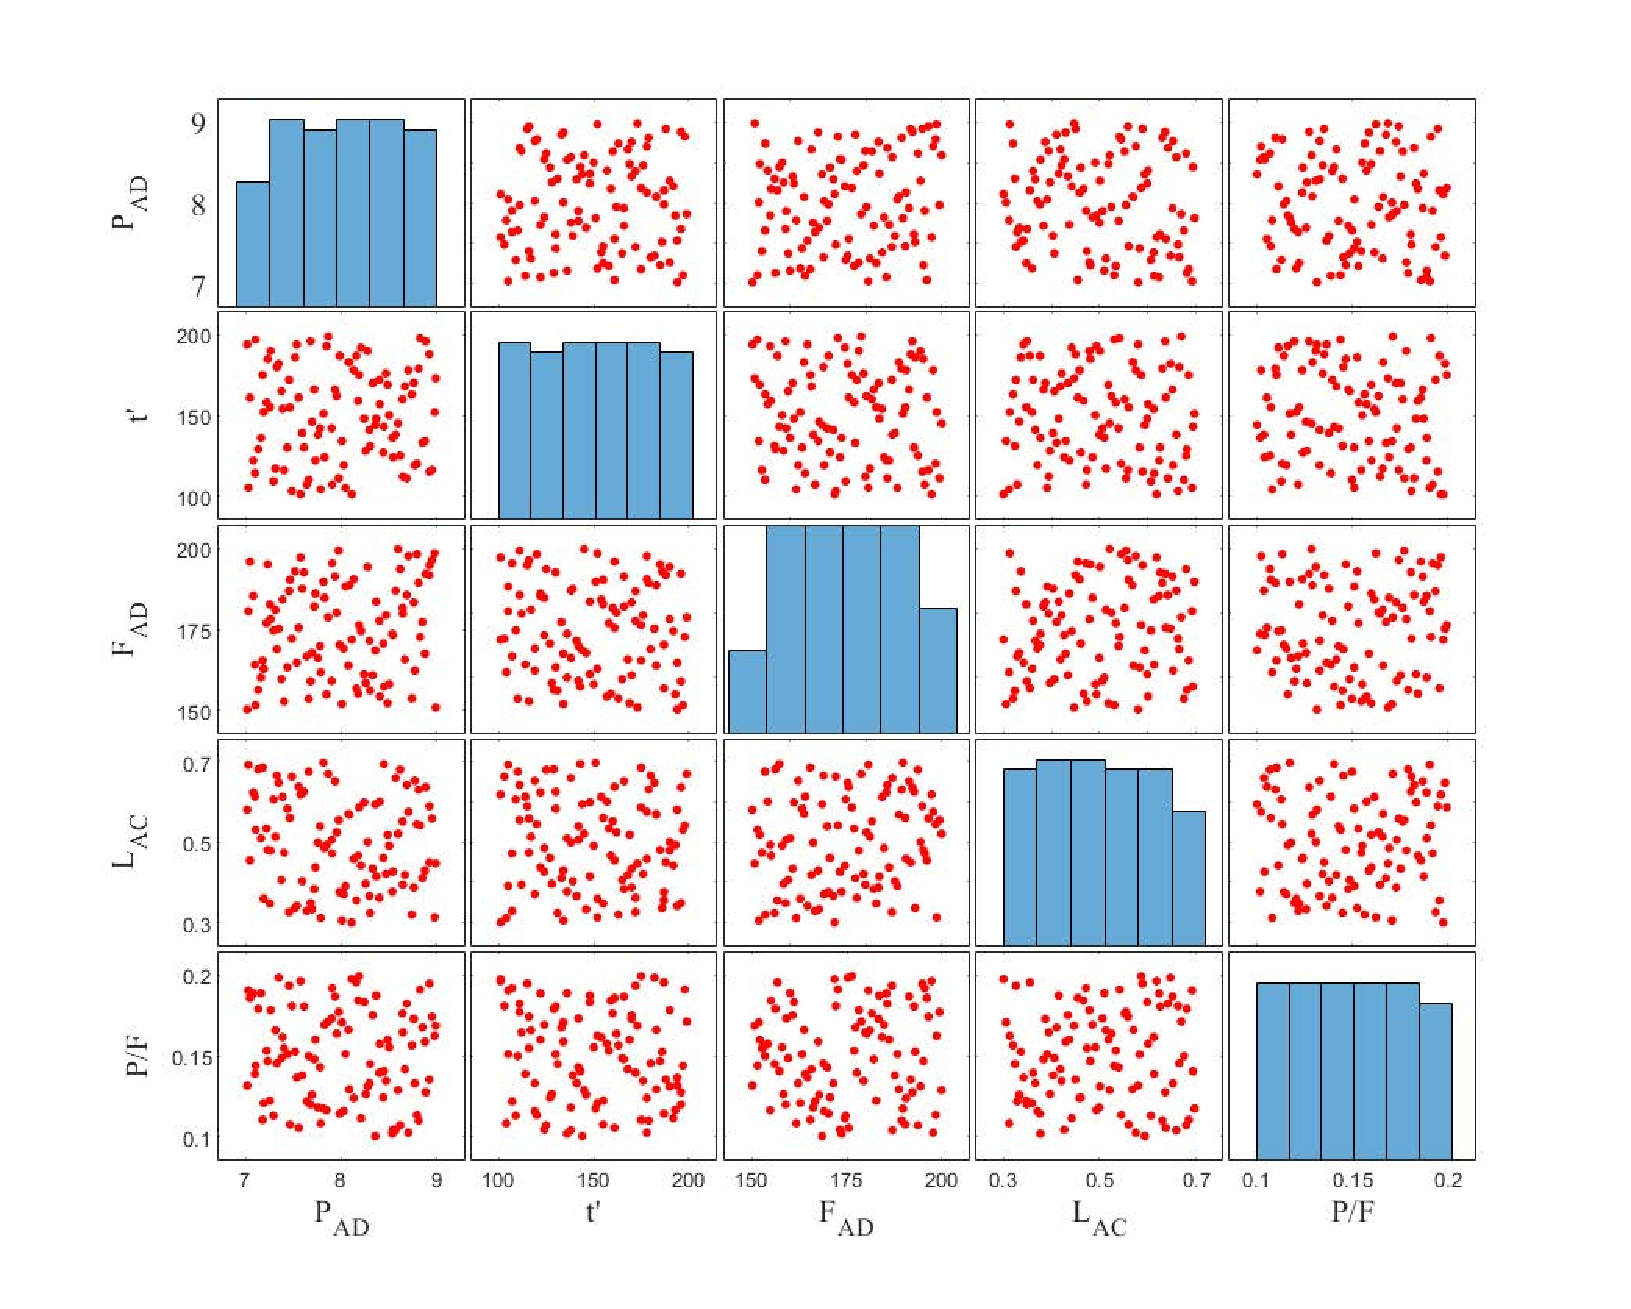
\includegraphics[width=1\textwidth]{figs/Fig4.pdf}
	\caption{Scatter plot matrix of decision variables}
	\label{FIG:4}
\end{figure}
\begin{figure}
	\centering
	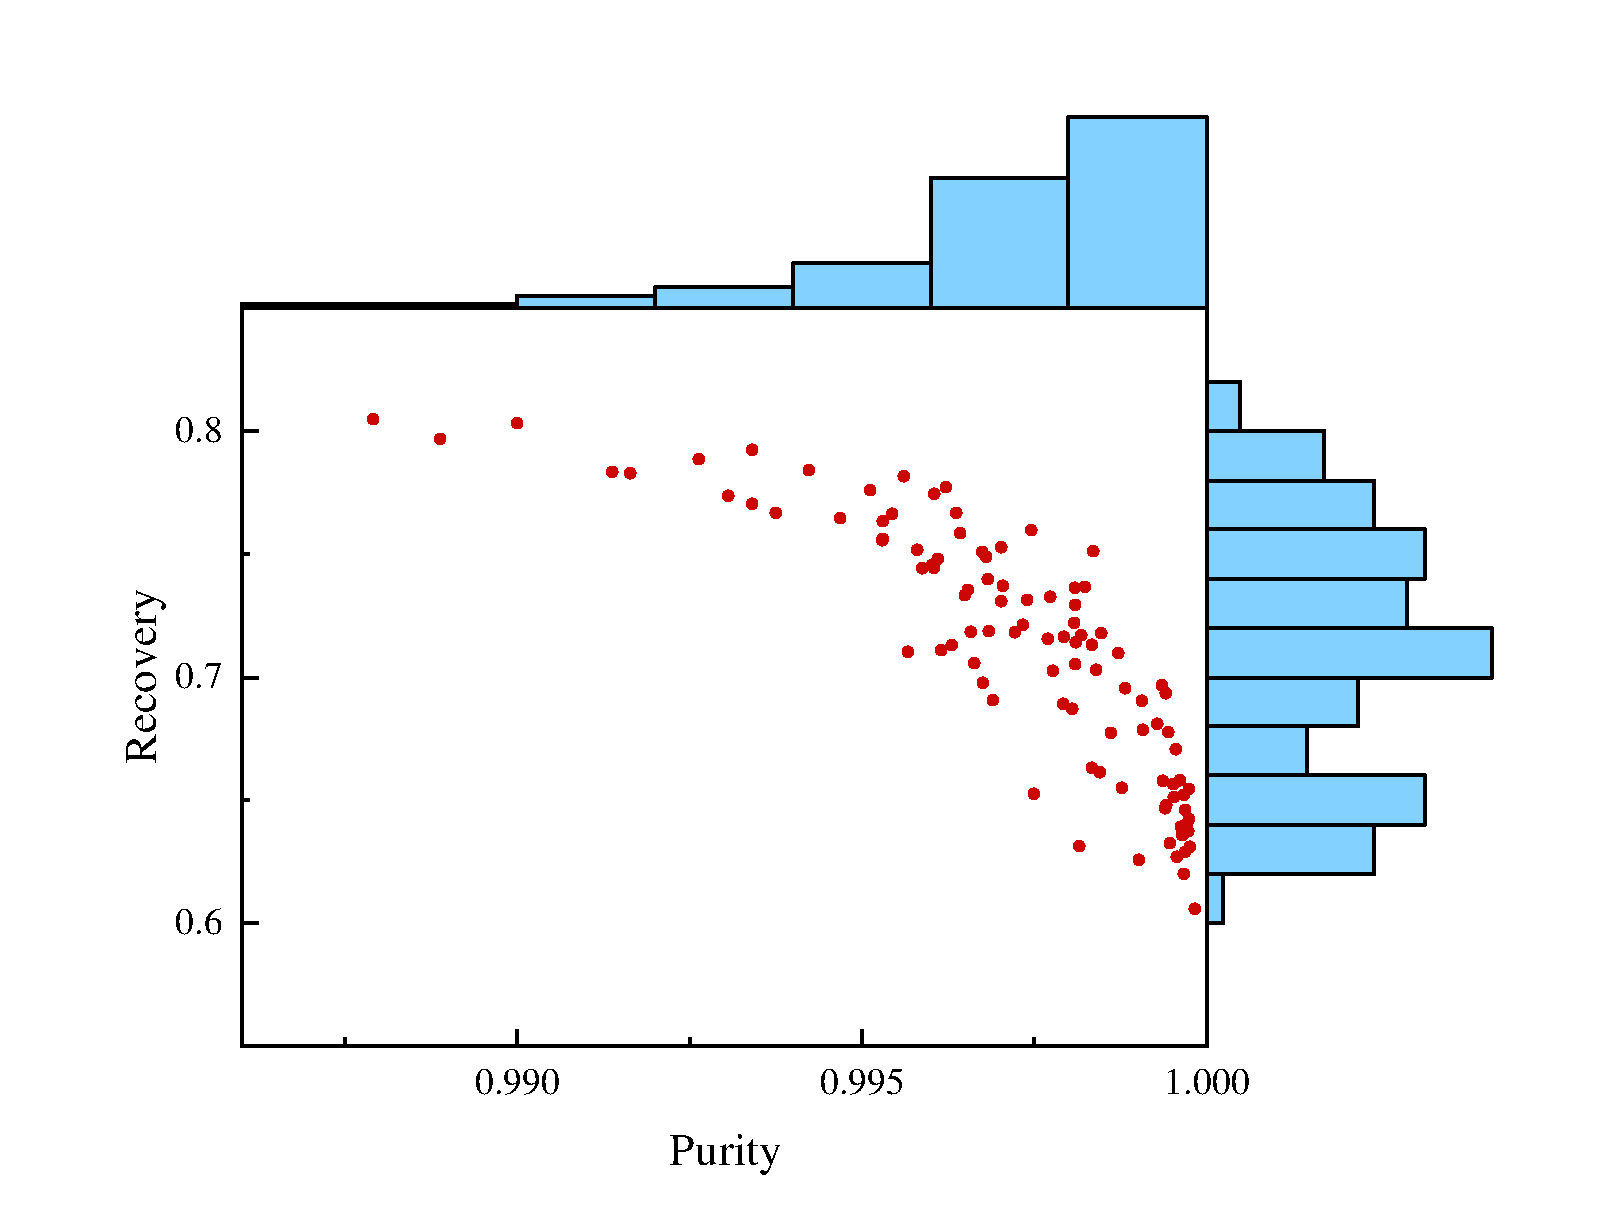
\includegraphics[width=0.7\textwidth]{figs/Fig5.pdf}
	\caption{Distribution of purity and recovery}
	\label{FIG:5}
\end{figure}

In order to ensure the efficient training and validation of the ANNs, we use Latin hypercube sampling (LHS) method for the generation of decision variables datasets of PSA simulator that is representative of the entire input space. This sampling strategy is a stratified sampling technique that adopts random sampling from a multi-dimensional parameter distribution and is often used in computer experiments, proposed by McKay et al\cite{RN51}. Five process variables were chosen as the decision variables and the inputs of ANN models, and the range of inputs conditions is shown as \cref{TABLE:3}. The pairwise relationship and distribution of multi-dimensional inputs is shown by scatter plot matrix, displayed in \cref{FIG:4}. The subplot in (i, j) of the matrix is a scatter plot of two different decision variables to represent the distribution at the projection surface. Along the diagonal are histogram plots of each decision variable to reveal the distribution frequency of data. What stands out in this figure is the uniform random distribution and there is no bias in the multi-dimensional space, which has shown the beneficial effects of ANN training. An sufficient database (100 samples) generated from the detail PSA model described in Section 3, is employed to train, validate and test the ANN. Purity, Recovery and Productivity are the performance indicators, and the distribution of purity and recovery is demonstrated in \cref{FIG:5}, the scatter plot shows the relationship and distribution of purity-recovery as well as the distribution of all the points has been demonstrated by histograms at two performance edges, the histograms reflect the proportion of the corresponding area (down or left). The marginal histograms plot illustrates the distribution of purity and recovery, and the highest purity and recovery reached 99.98\% and 80.48\% respectively among all the samples. Most of the points are concentrated in the high purity area, and the recovery is relatively uniform. The detailed results have been summarised in Table S4 and Fig.S3.
\section{ANN-based surrogate models: training and validation}
Owing to the great predictive and fitted abilities over a set of reports, ANNs have excellent performance for working as the surrogate models, mentioned before in section 1. ANN, used in this work, is a nonlinear regression model that consists of multi layers: input layer, output layer and several hidden layers. An ANN with none hidden layer is only capable to approximate a linear system. However, if there were one hidden layer, it could represent any function that contains a continuous relationship between inputs and outputs. Considering the complexity of the PSA process, the ANNs designed as the surrogate models should have one hidden layer. Otherwise, in consideration of a set of neurons in each layer, the number of neurons in input and output layer is equal to the number of inputs and outputs, respectively. And the number of neurons in the hidden layer affects the accuracy of ANN fitting, using too few neurons in the hidden layer will result in underfitting. Oppositely, using too many neurons will increase the training time or lead to overfitting, which makes it difficult to achieve the expected performance. However, how to determine the number of neurons in the hidden layer is still an unresolved problem. In practical applications, it is usually adjusted by empirical formulas with trial and error \cite{RN52}.In this work, we refer to two empirical formulas, \cref{num1} [19] and \cref{num2} \cite{RN53}, to determine the number of neurons in the hidden layer combined with trial and error, and it is set to 8.
\begin{equation}
	{N_h} = 2{N_s} + 1\label{num1}
\end{equation}
\begin{equation}
	{N_h} = \frac{{{N_s}}}{{\left( {\alpha  * \left( {{N_i} + {N_o}} \right)} \right)}}\label{num2}
\end{equation}
Where Ns is the numbers of training samples, Ni, Nh, and No is the number of input layer, hidden layer, and output layer, respectively.
In this work, two different multi-layer feedforward neural networks with error backpropagation algorithm are used as the surrogate models. The \cref{ann} and \cref{gaiddown} are the calculation method of back propagation artificial neural network [52].Detailed parameters of ANNs have been demonstrated in \cref{TABLE:4} and the architecture of ANNs is shown in \cref{FIG:6}. The nonlinear relationship between input and output is approximated by the following equations:
\begin{equation}
	\begin{array}{l}
		{\alpha _h} = \sum\nolimits_{i = 1}^d {{v_{ih}}{x_i} + {b_h}} \\
		{\beta _h} = \frac{1}{{1 + {e^{ - {\alpha _h}}}}}\\
		{\alpha _o} = \sum\nolimits_{h = 1}^q {{w_{ho}}{\beta _h} + {b_o}} \\
		{\beta _o} = {\alpha _o}
	\end{array}\label{ann}
\end{equation}
Here, $\aleph$ and $\beta$ stands for input and output respectively; vih and who are the connection weight of input-hidden and hidden-output; x is the input vector and b is the node bias of a certain neuron; d and q are the number of neurons in the input layer and hidden layer, separately. Subscript h and o represent the neuron of hidden layer and output layer.

The mean square error (MSE) is used to estimate the connection weights and biases based on gradient descent method:
\begin{equation}
	\begin{array}{l}
		{\widehat y_i}^k = f({\alpha _o})\\
		{E_k} = \frac{1}{n}\sum\nolimits_{i = 1}^q {{{({{\widehat y}_i}^k - {y_i}^k)}^2}} \\
		\Delta {w_{ho}} =  - \eta \frac{{\partial {E_k}}}{{\partial {w_{ho}}}}\\
		{w_{ho}} \leftarrow {w_{ho}} + \Delta {w_{ho}}
	\end{array}\label{gaiddown}
\end{equation}
$\widehat y$ in \cref{gaiddown} is the results of ANN, the output of the nodes in output layer, and the calculation method has been added to \cref{gaiddown}. While the purelin has been applied as the activation function of output layer, f is y=x and the output of ANN equal to $\beta$o, shown in \cref{ann}. y is the target output and $\eta$ is the learning rate given.


\begin{table}[]
	\centering
	\caption{Structural parameters of artificial neural networks}
	\begin{tabular}{lll}
		\toprule
		& ANN1                             & ANN2               \\
		\midrule
		Inputs   (X)              & \multicolumn{2}{l}{PAD;   t'; FAD; LAC;P/F}           \\
		Outputs   (Y)             & Purity;   Recovery; Productivity & Purity;   Recovery \\
		The number of …           & \multicolumn{2}{l}{}                                  \\
		Neurons   of input layer  & \multicolumn{2}{l}{5}                                 \\
		Neurons   of hidden layer & \multicolumn{2}{l}{8}                                 \\
		Neurons   of output layer & 3                                & 2                  \\
		Activation function of …  & \multicolumn{2}{l}{}                                  \\
		Hidden   layer            & \multicolumn{2}{l}{sigmoid}                           \\
		Output   layer            & \multicolumn{2}{l}{purelin}                          \\
		\bottomrule
	\end{tabular}
\label{TABLE:4}
\end{table}
\begin{figure}
	\centering
	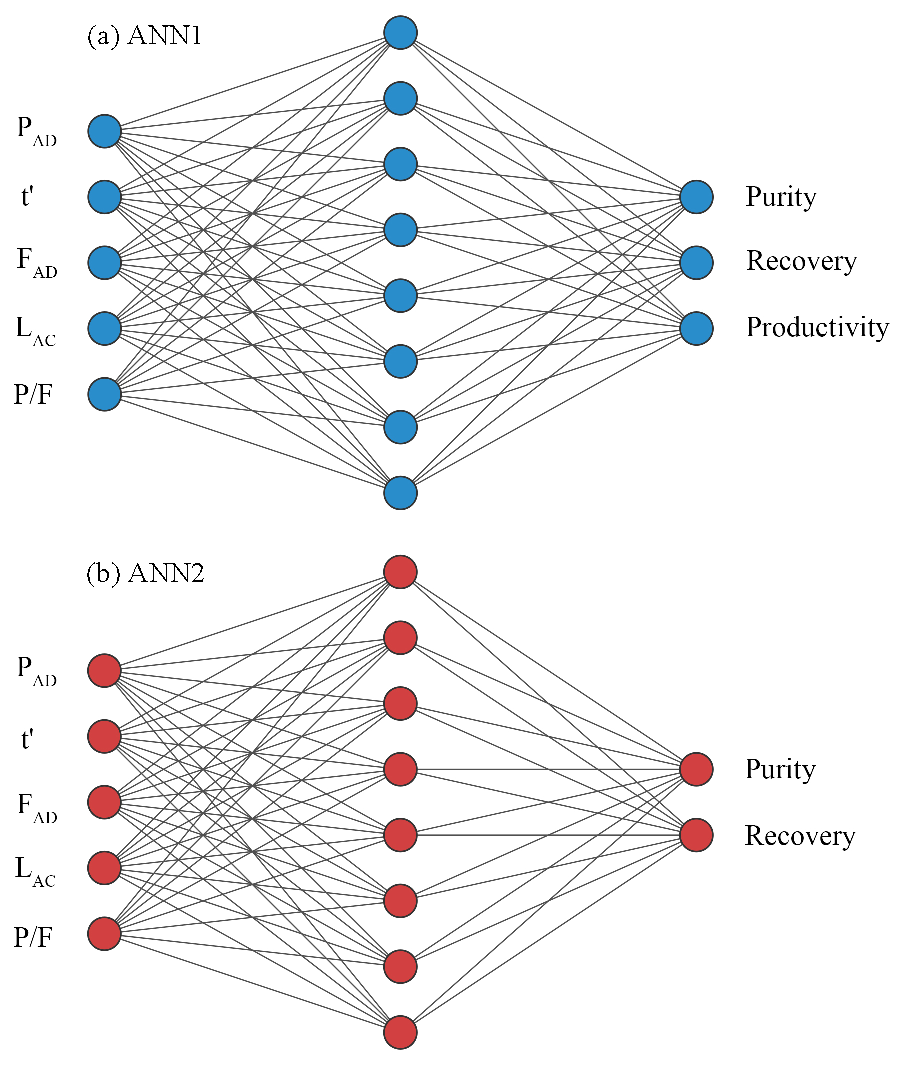
\includegraphics[width=1\textwidth]{figs/Fig6.pdf}
	\caption{Architectures of (a) ANN1 and (b) ANN2}
	\label{FIG:6}
\end{figure}
As shown in Table S4, the database, generated by LHS Strategy and calculated using detail PSA models in Section 3, is randomly split into three sets: Training set, Validation set and Testing set, with a proportion of 6:2:2. Training set is used to adjust the connection weights and biases by above mentioned MSE method during training; samples of validation are applied to determine the network structure and halt training to avoid overfitting; testing set does not work on training but is an independent measure for testing the performance of the optimal ANN model. Depending on the sample sets above, we have trained two multi-layer feedforward neural networks with error backpropagation algorithm on the basis of Levenberg-Marquardt method in MATLAB.

From the data in \cref{FIG:5}, the purity and recovery of this PSA process are very high, especially purities are extremely close to 1. Therefore, the purity predicted by ANNs could be greater than 1 under some operating conditions. To avoid the approximation of surrogate models exceeds the physical boundary and enhance the robustness of the ANNs, an output transformation has been applied to impose the prediction of purity and recovery falls in the boundaries by \cref{ytransfor}:
\begin{equation}
	\begin{array}{l}
		u =  - \frac{1}{\zeta }\log \left[ {{{\left( {\frac{{k - x}}{{y - x}}} \right)}^\nu } - 1} \right]\\
		\widehat y = x + \frac{{k - x}}{{{{(1 + \exp ( - \zeta  * \widehat u))}^{\frac{1}{v}}}}}
	\end{array}\label{ytransfor}
\end{equation}
Where u is the transformed value of output, k and x are respectively the upper and lower asymptotic boundary, $\zeta$ and v are constants. $\widehat y$ is the prediction transformed back. When performing multi-objective optimization, the transformed output data can keep the Pareto ordering unchanged\cite{RN32}. Many researchers use similar transformation methods as an essential ingredient\cite{RN29,RN32,RN54}.

\begin{table}[]
	\centering
	\caption{Training results of two artificial neural networks}
	\begin{tabular}{lll}
		\toprule
           & MSE         & R        \\
           \midrule
			\multicolumn{3}{l}{ANN1}            \\
			Training   & 1.01630E-04 & 0.999958 \\
			Validation & 1.80110E-04 & 0.999917 \\
			Testing    & 9.74971E-05 & 0.999956 \\
			All        & 1.16419E-04 & 0.999950 \\
			\multicolumn{3}{l}{ANN2}            \\
			Training   & 1.95383E-07 & 0.999995 \\
			Validation & 3.09196E-06 & 0.999927 \\
			Testing    & 3.15566E-06 & 0.999926 \\
			All        & 1.36581E-06 & 0.999970\\
		\bottomrule
	\end{tabular}
\label{TABLE:5}
\end{table}
\begin{figure}
	\centering
	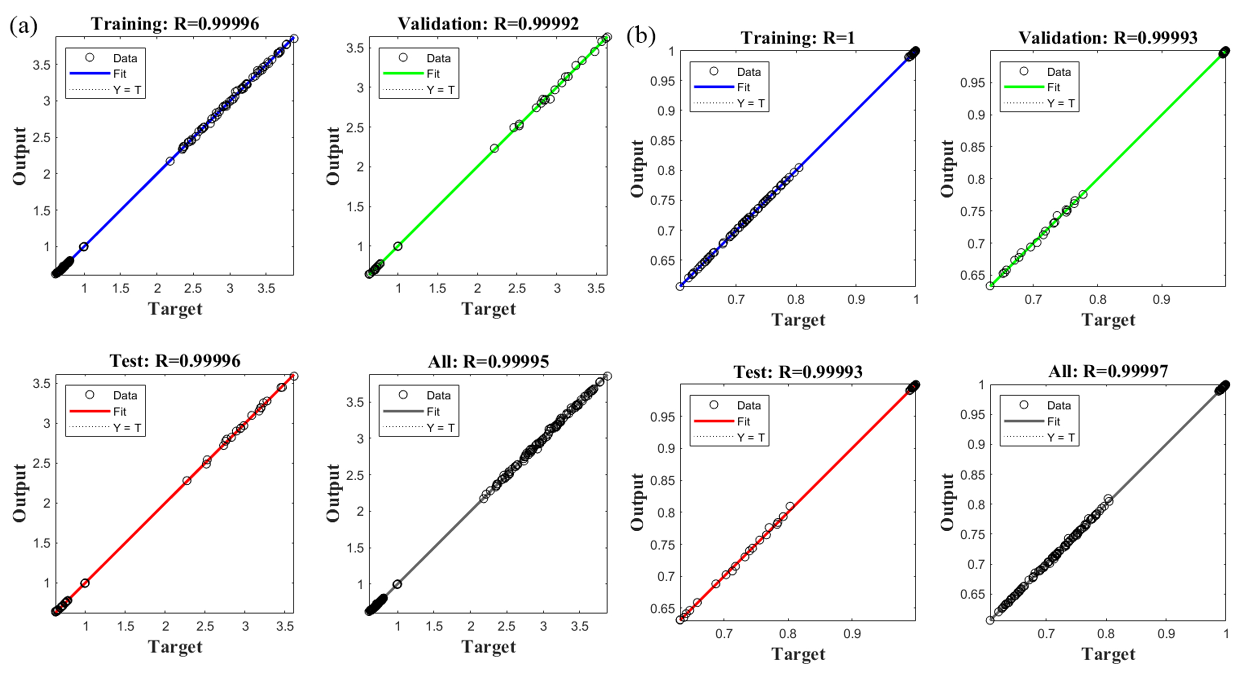
\includegraphics[width=1\textwidth]{figs/Fig7.pdf}
	\caption{Regression correlation coefficients between Detailed models and ANN-based surrogate models: (a) ANN1; (b) ANN2}
	\label{FIG:7}
\end{figure}

The performance and regression accuracy are judged by MSE and R values. MSE and regression R reflects the error and the correlation between the predicted outputs and the targets. The datasets of PSA process performance indicators, purity, recovery, and productivity, are generated from different models, including Detailed models, ANN1 and ANN2, shown in Table S5. Training results of both ANNs are displayed in \cref{TABLE:5} and \cref{FIG:7}. The overall training effects of PSA process performance for hydrogen purification achieve 0.999950 and 0.999970, respectively, and excellent training performance can be seen in \cref{FIG:7}. The results of the correlational analysis highlight that the artificial neural networks can fit and predict the PSA process with extremely high accuracy, so it can be employed as surrogate models for the next optimization.

\section{Process optimization using ANN-based surrogate models}
\begin{figure}
	\centering
	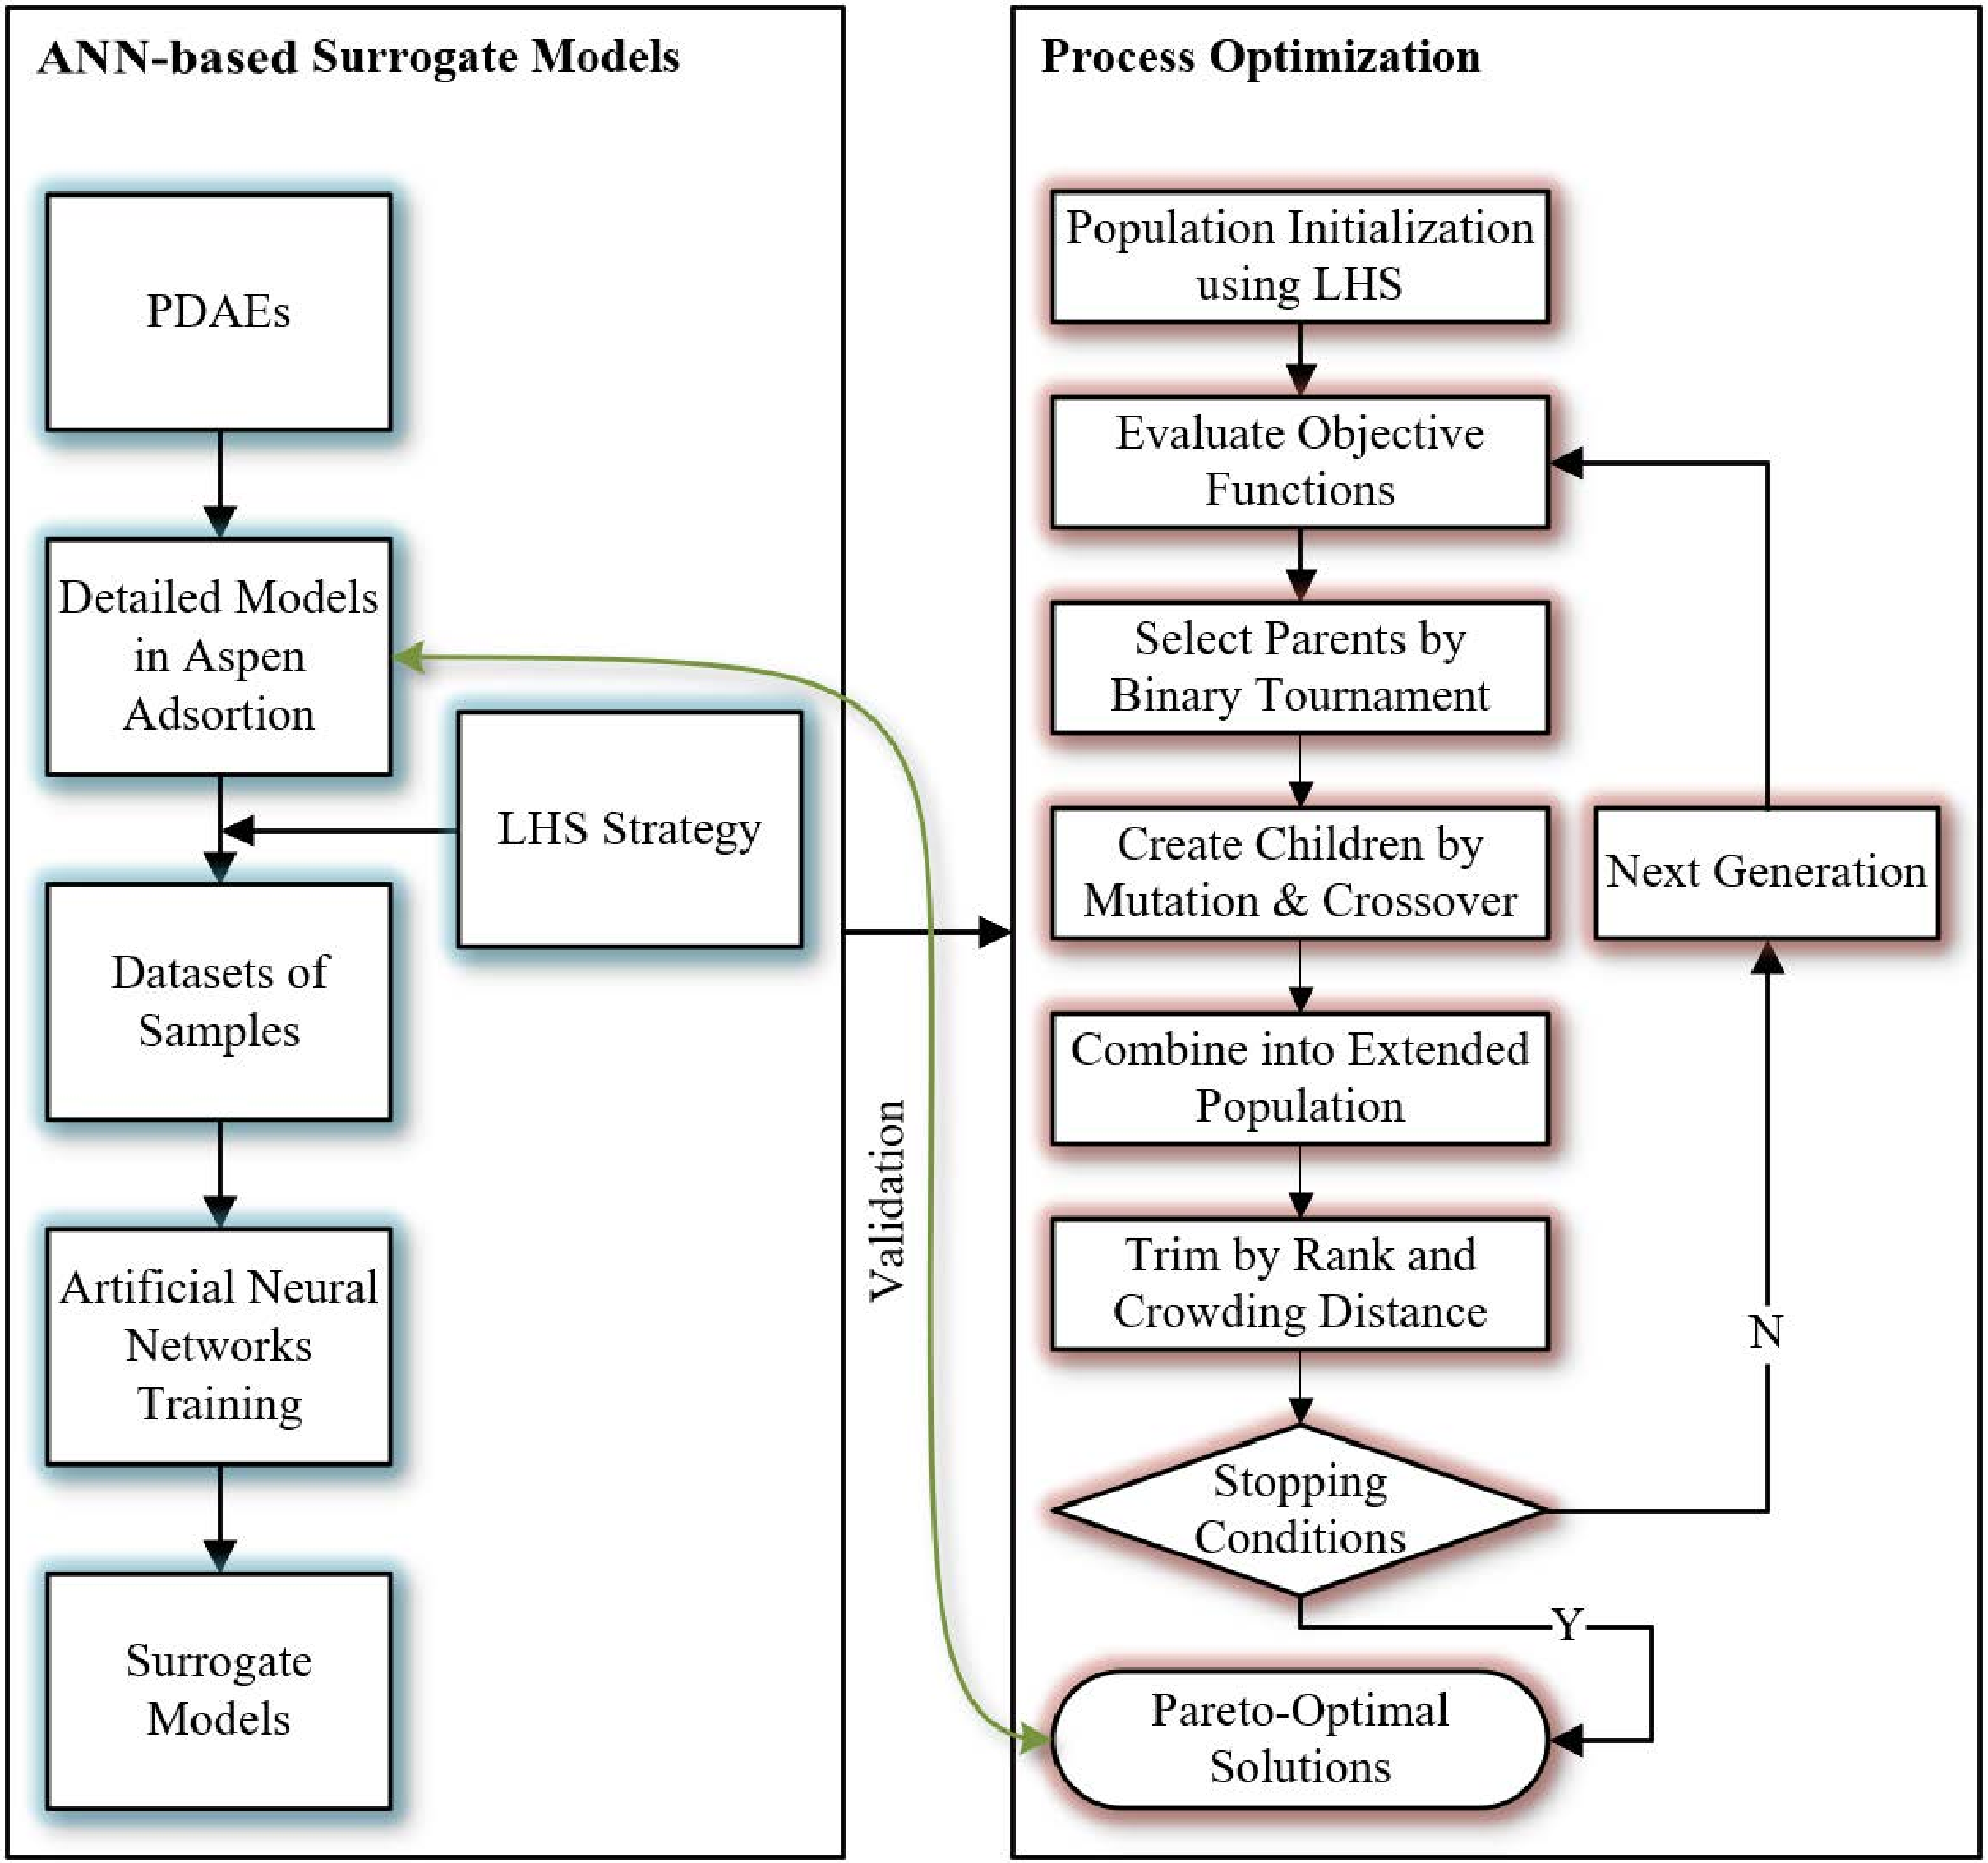
\includegraphics[width=1\textwidth]{figs/Fig8.pdf}
	\caption{Procedure of multi-objective optimization of ANN-based PSA surrogate models}
	\label{FIG:8}
\end{figure}
In a PSA process, several process targets could be regarded as the performance indicator. The goals are maximizing the process productivity, minimization of energy consumption and improving purity and recovery of product as much as possible. It is ideal to achieve these purposes, but there are competing and conflicting relationship among them, i.e., higher purity causes lower recovery. And it is prerequisite to satisfy the specified goal of purity and recovery, along with optimizing the other variables. Therefore, multi-objective optimization is formulated for the PSA optimization problem, and it is vital to choose the optimization objective function\cite{RN55}. In this work, purity, recovery and productivity are selected as the objective function of the optimization problem, and two typical multi-objective optimization problems using the ANN-based surrogate models of PSA process are performed: (1) Dual-objective optimization: purity and recovery are the objective functions; (2) Tri-objective optimization: productivity is used as an additional objective. The Non-dominated sorting genetic algorithm-\uppercase\expandafter{\romannumeral2} (NSGA-\uppercase\expandafter{\romannumeral2}) is employed to pursue a set of feasible solutions, namely the Pareto-Optimal Front. The schematic of the optimization process with NSGA-\uppercase\expandafter{\romannumeral2} is shown as \cref{FIG:8} and implemented as follows: the ANNs have been well trained as mentioned in section 5 and applied as surrogated models in process optimization; a set of decision variables have been extracted from the multi-dimensional parameter distribution using LHS as the initial population and sorted based on non-domination; parents are selected by using binary tournament selection and generates children by crossover and mutation; the worse half individuals are trimmed based on rank and crowding distance on the last front; the pareto-optimal solutions will be validated by the Detailed models.

We use spread to measure the movement of pareto improvement, calculated by \cref{spread}.
\begin{equation}
	spread = \frac{{\mu  + \sigma }}{{\mu  + Qd}}\label{spread}
\end{equation}
Where $\mu$ is the sum of the difference of the objective functions between last two iterations. The crowding distance of the two endpoints at the Pareto front is infinite, other points with finite distance are used to calculate parameters $\sigma$, Q and d, represented the standard deviation of the crowding distance, the number of these points and the average distance measure among them. When the objective function value changes slightly much between several iterations or the points on the Pareto front line are evenly distributed, the value of spread is low\cite{RN56}.
\begin{table}[]
	\centering
	\caption{Parameters of the Evolutionary Algorithm Optimization}
	\begin{tabular}{llll}
		\toprule
		& \multicolumn{2}{l}{\begin{tabular}[c]{@{}l@{}}Dual-objective   \\ optimization\end{tabular}} & {\begin{tabular}[c]{@{}l@{}}Tri-objective   \\ optimization\end{tabular}} \\
		\midrule
		PopulationSize      & \multicolumn{2}{l}{100}                           & 1000                         \\
		ParetoFraction      & \multicolumn{2}{l}{0.20}                          & 0.35                         \\
		Initialpopulation   & \multicolumn{3}{l}{100 Samples of Training}                                      \\
		FunctionTolerance   & 1e-4                      & \multicolumn{2}{l}{1e-5}                             \\
		MaxStallGenerations & \multicolumn{3}{l}{100}                                                          \\
		MaxGenerations      & \multicolumn{3}{l}{2000}                                                         \\
		MaxTime             & \multicolumn{3}{l}{3600}                                                         \\
		CrossoverFraction   & \multicolumn{3}{l}{0.8}                                                         \\
		\bottomrule
	\end{tabular}
\label{TABLE:6}
\end{table}
The stopping conditions settled include: (1) Stall generations: the value of spread over specific number of generations (MaxStallGenerations) is less than tolerance (FunctionTolerance), and the spread of last generation is less than the mean spread of these generations; (2) Generations: reached the maximum number of generations; (3) Time limit: the process reaches to the maximum time specified. Other parameters of the algorithm in two different optimizations are demonstrated in detail as \cref{TABLE:6}. The function tolerance of Dual/Tri-objective optimization are 1e-4 and 1e-5, which are determined by the recommendation of Global Optimization Toolbox Documentation \cite{RN57} and our experience value, which could meet the accuracy requirements of optimization work and perform well.

In this study, the optimization using NSGA-\uppercase\expandafter{\romannumeral2} is achieved in MATLAB, and the main optimization goal is to maximize purity, recovery, and productivity. Due to the trade-off between objective functions, we pursue a series of feasible points using Pareto technology. Hydrogen is used in many fields, such as petroleum cracking, ammonia synthesis and fuel cells, whose applications basically require the purity to be greater than 99\%\cite{RN58}, so this performance index is handled as a constraint into this problem. In addition, the reason why energy consumption is not set as an objective function is that it is directly related to pressure of adsorption in the normal temperature PSA process without a vacuum step\cite{RN11} and is limited by decision variables and process parameters. Five process variables, PAD, t', FAD, LAC and P/F are chosen as the decision variables and the range is shown as \cref{TABLE:3}.

\subsection{Dual-objective optimization}
The ANN1 which has five inputs (Xi: [PAD, t’, FAD, LAC,P/F]) and two outputs (Yi:[Purity, Recovery]) could be formulated as: Yi=fANN1(Xi). The accuracy of this input-output relationship is indicated by the mean square error and regression R, 1.16419E-04 and 0.999950 for total each, shown in \cref{TABLE:5} and \cref{FIG:4}. Therefore, the ANN1 has such an extremely high accuracy that is suitable for the Dual-objective optimization, formulated as:
\begin{displaymath}
	\begin{array}{l}
		Maximize:     Purity, Recovery\\
		Subject to:      {Y_i} = {f_{ANN1}}({X_i})\\
		Purity \ge 99\% \\
		{X_i} \in [lb,ub] 
	\end{array}
\end{displaymath}
\begin{figure}
	\centering
	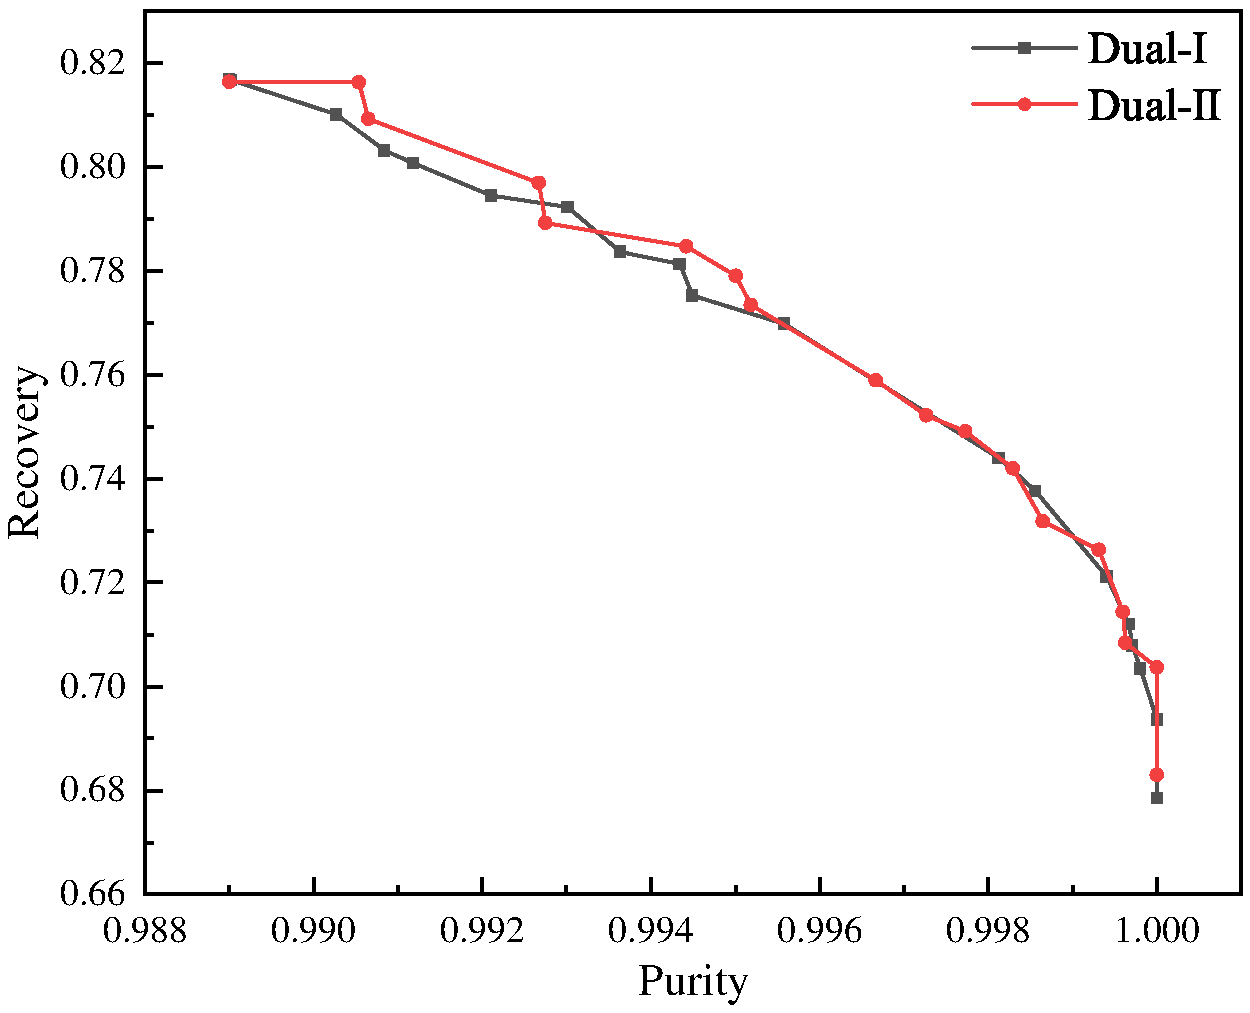
\includegraphics[width=0.5\textwidth]{figs/Fig9.pdf}
	\caption{Pareto-Optimal Fronts of Dual-objective optimization}
	\label{FIG:9}
\end{figure}
\begin{figure}
	\centering
	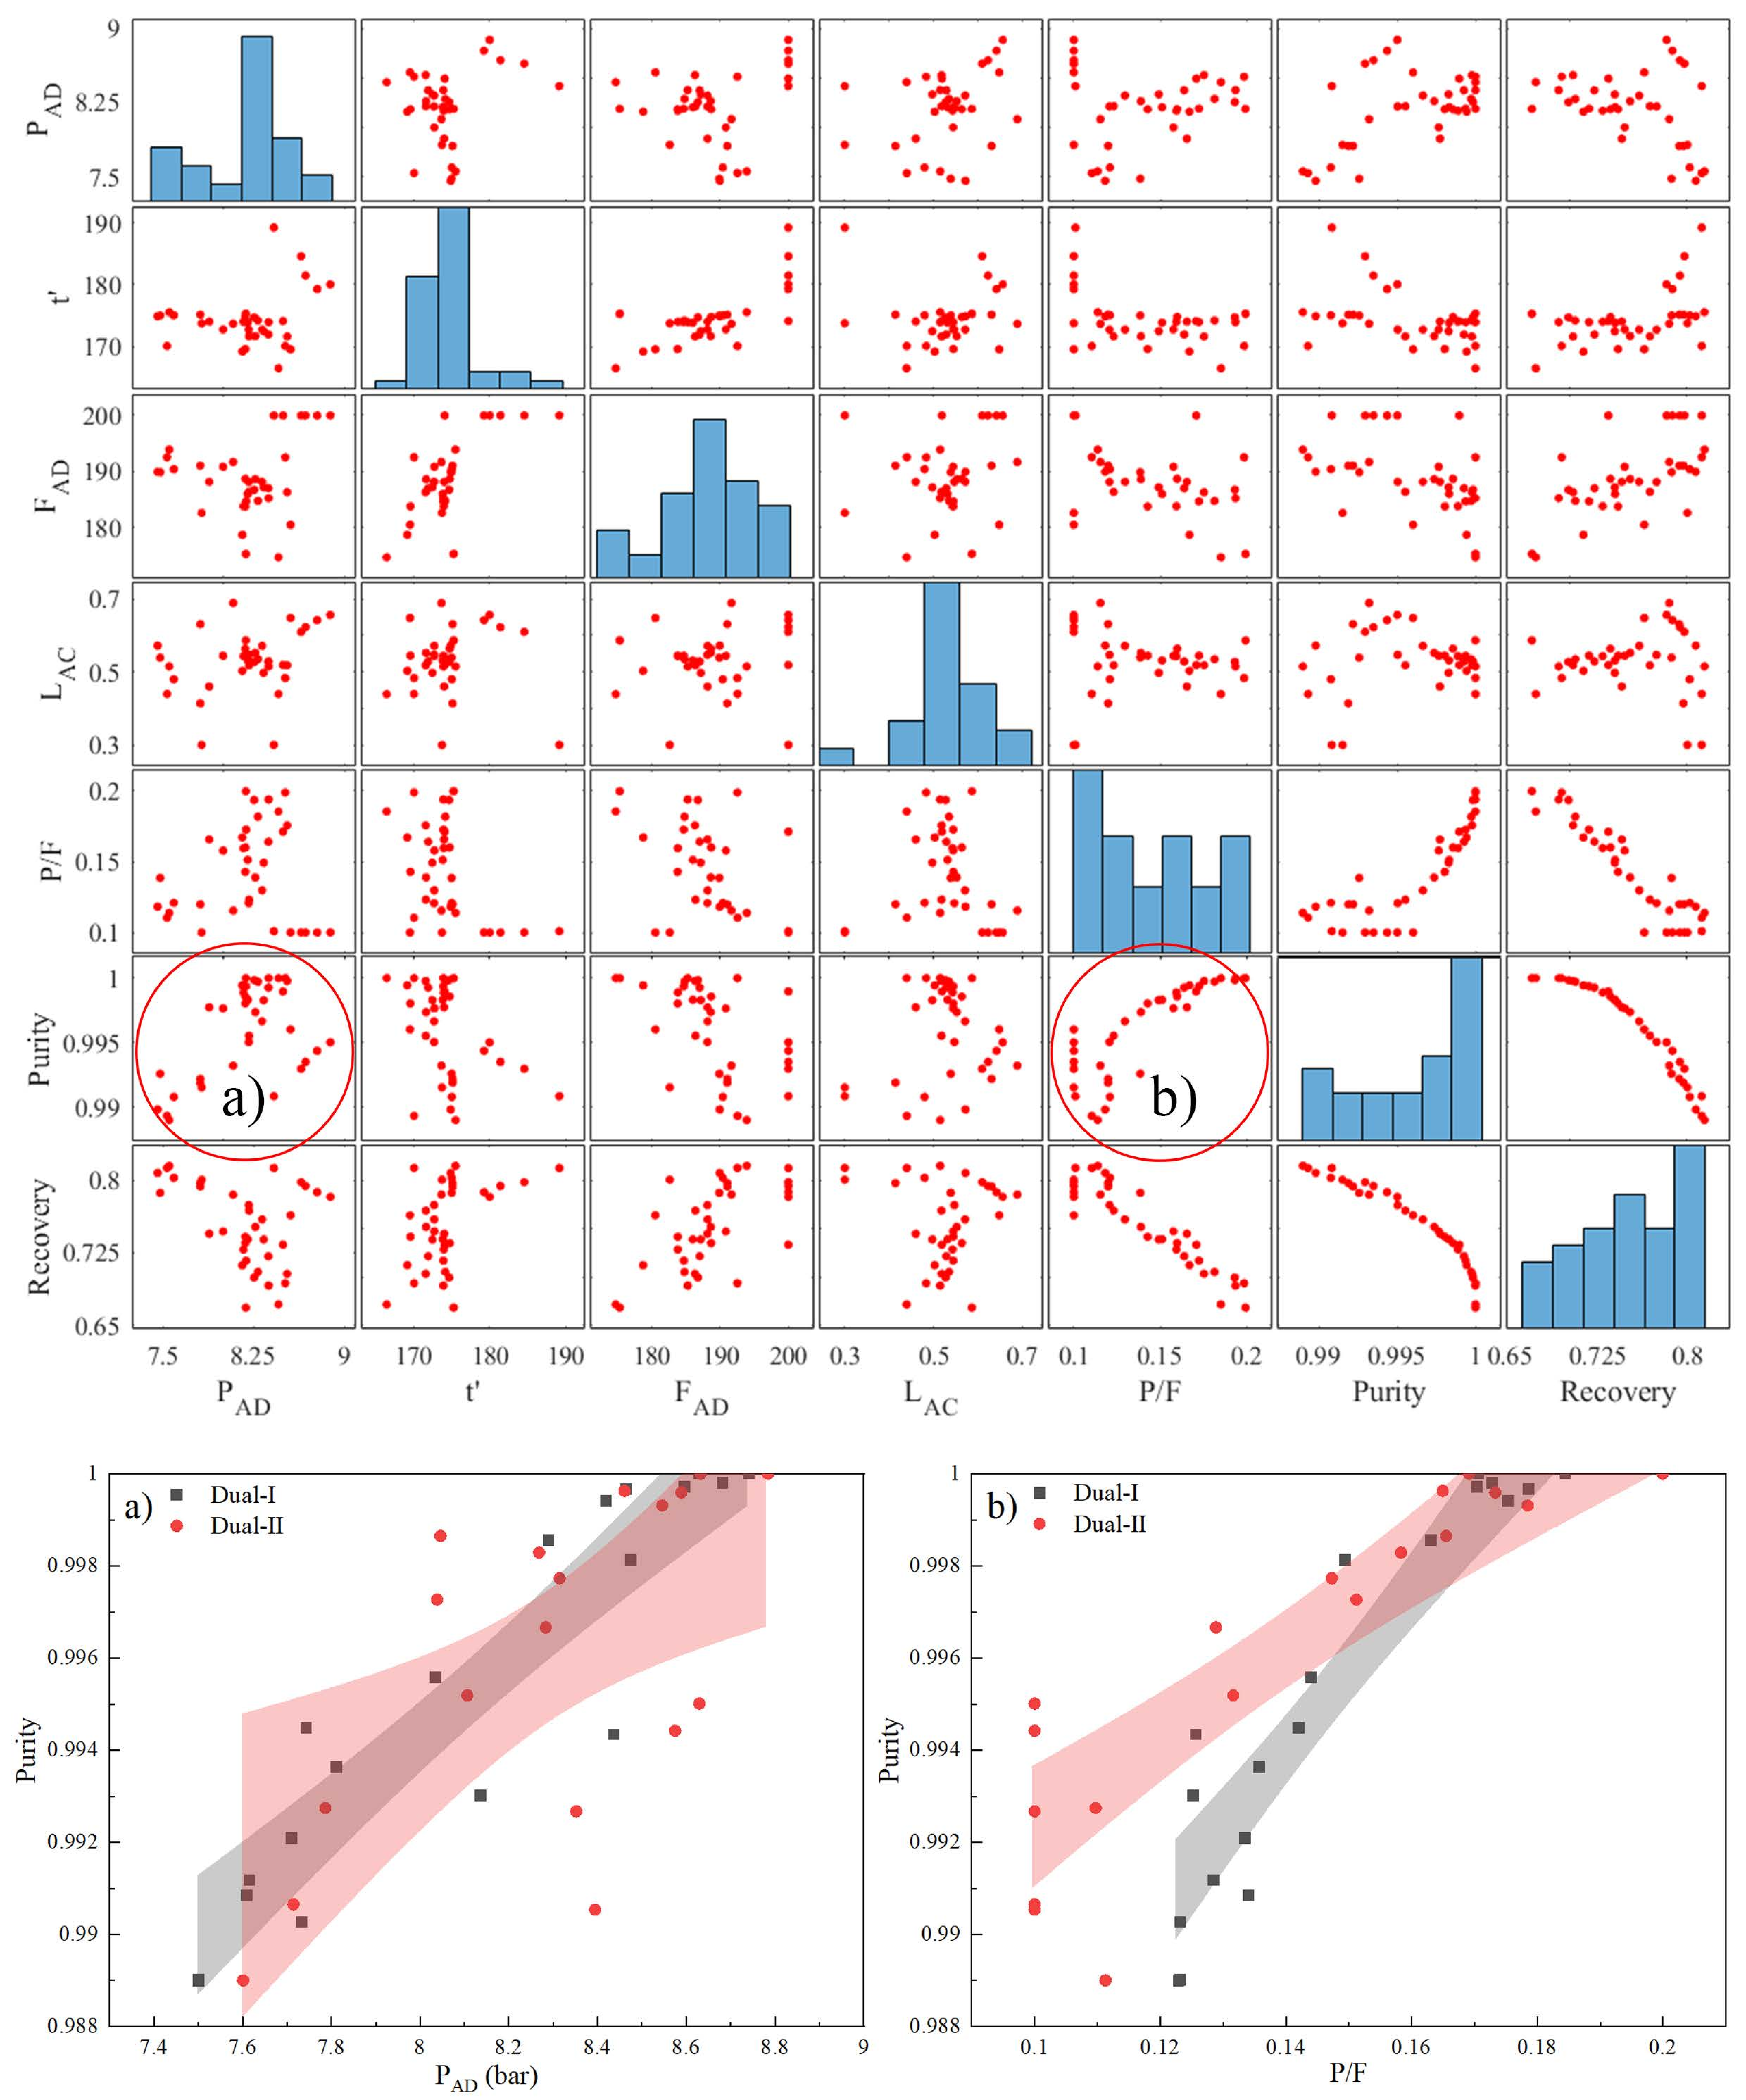
\includegraphics[width=1\textwidth]{figs/Fig10.pdf}
	\caption{The relationship between objective function and decision variables in both two Pareto-Optimal Fronts; the 95\% confidence band of each set of data is represented by the shaded area: (a) Purity-PAD; (b) Purity-P/F ratio}
	\label{FIG:10}
\end{figure}
In this optimization, we have used two different methods to find the pareto-optimal front: (1) Dual-\uppercase\expandafter{\romannumeral1}: compute this problem using NSGA-\uppercase\expandafter{\romannumeral2} only; (2) Dual-\uppercase\expandafter{\romannumeral2}: combining with the hybrid function, which is a formulation for minimizing a multiobjective optimization problem with different wights and applied after the NSGA-\uppercase\expandafter{\romannumeral2} completed[56]. The detailed solving procedure of the latter is interpreted in Supporting Information. The pareto-optimal fronts of both methods are displayed as \cref{FIG:9}, and Table S6 enumerates two sets of data obtained from two optimizations and the simulation results using Detailed models for validation of all the points in Pareto-Optimal Fronts. The accuracy is calculated by \cref{accuracy}. The number of optimal solutions is equal to the PopulationSize multiplied by the ParetoFraction, and it is worth noting that there are one or two repeated solutions due to the characteristics of the meta-heuristic algorithm. In the optimal sets, the relationships between different decision variables and the objective functions are displayed as \cref{FIG:10} to further verify the rationality of the results.
\begin{equation}
	Accuracy (\% ) = \frac{{\left| {{y_{opt}} - {y_{detailed}}} \right|}}{{{y_{detailed}}}} \times 100\% \label{accuracy}
\end{equation}
As can be seen from the above result: The Dual-\uppercase\expandafter{\romannumeral2} method is slightly better than the Dual-\uppercase\expandafter{\romannumeral1} at the top left of the \cref{FIG:9}. Because the PSA process has greater operating flexibility at low purity for further optimization, but it is difficult to improve when the purity is extremely high and close to 1. After simulating each point on the Pareto front using Detailed models and comparing the results of simulation and prediction, it can be found that there is almost no difference with higher than 99\% accuracy as shown in Table S6, which thanks to the high-precision ANN-based surrogated models. The average accuracy of purity and recovery in pareto-optimal solutions are 99.91\% and 99.82\% for Dual-\uppercase\expandafter{\romannumeral1}, 99.95\% and 99.68\% for Dual-\uppercase\expandafter{\romannumeral2}, respectively. \cref{FIG:10} displays the intercorrelations among all these variables of two datasets of pareto-optimal solutions. The relations of Purity-PAD and Purity- P/F ratio have been pick up from the overall matrix to figure a and b, several important laws can be observed in \cref{FIG:10}: higher adsorption pressure leads to higher purity; the reduction in P/F ratio could save the H2 consumption during the Purge step and increase recovery; there is a tradeoff between purity and recovery, all of which are in line with the general disciplines of the PSA process. A few points fall outside the confidence band because the objective function is also affected more strongly by the other four variables. A comprehensive analysis of each two methods is shown in the Supporting Information as Fig.S4 and Fig.S5, respectively. Therefore, the results indicate that the ANN1-based surrogated model is suitable for the dual-objectives optimization using genetic algorithm, including NSGA-\uppercase\expandafter{\romannumeral2} and NSGA-\uppercase\expandafter{\romannumeral2} with hybrid function. The two sets of pareto-optimal solutions are feasible and can be used as a basis for selection of process conditions for improvement.
\begin{table}[]
	\centering
	\caption{Parameters of the Cases for optimization evaluating}
	\begin{tabular}{llllllll}
		\toprule
		& \multicolumn{2}{l}{PAD   (bar)} & FAD   (SLPM) & LAC   (m) & P/F   & Purity & Recovery \\
		\midrule
		Case   A & \multicolumn{2}{l}{7.501}       & 197.97       & 0.4022    & 1.229 & 0.9894 & 0.8198   \\
		Case   B & \multicolumn{2}{l}{8.632}       & 172.87       & 0.5224    & 1.691 & 0.9997 & 0.6856  \\
		\bottomrule
	\end{tabular}
\label{TABLE:7}
\end{table}
\begin{figure}
	\centering
	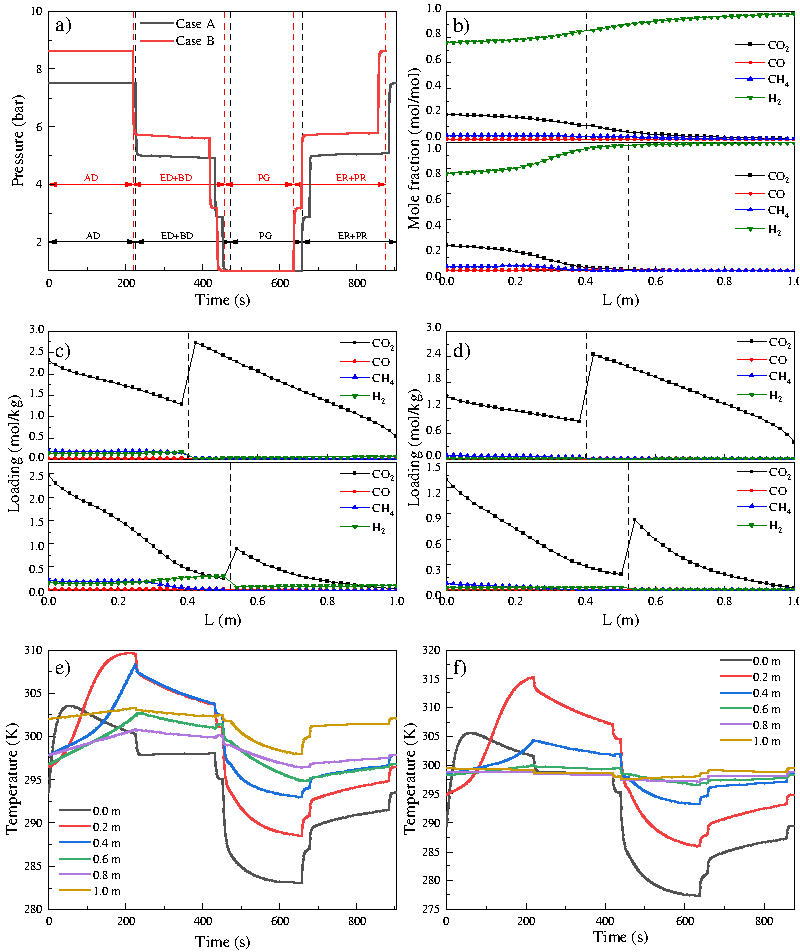
\includegraphics[width=1\textwidth]{figs/Fig11.pdf}
	\caption{Dynamic and Transmitted behaviors of PSA process at CSS: a) Pressure profiles under Case A \& B; b) gas phase concentration profiles at the end of AD step; c) solid phase loading at the end of AD step; d) solid phase loading at the end of PG step; e) \& f) Temperature profiles under Case A \& B. (In fig b, c and d, A is the above and B is the below)}
	\label{FIG:11}
\end{figure}
To evaluate the optimization results, the dynamic and transmitted behaviors of PSA process have been obtained under the operating conditions of the two end points in Pareto-Optimal Fronts, case A and case B, the detailed parameters are summarised in \cref{TABLE:7}. The pressure profile during a cycle as well as the gas/solid phase concentration and temperature profiles along the bed at CSS are set out in \cref{FIG:11}.

As shown in \cref{FIG:11}a and \cref{TABLE:7}, case B has higher adsorption pressure as well as lower feed flowrate and adsorption time to achieve ultra-purity H2. Looking at \cref{FIG:11}b, it is apparent that most impurities have been adsorbed almost at the end of bed in case A and at 0.5 m in case B, which can give rise to a higher overall recovery and the greater H2 purity at outlet, respectively. What stands out in \cref{FIG:11}c and \cref{FIG:11}d is the adsorption and desorption performance along two layers, the adsorption amount of CO2 along the bed in case A is significantly higher which cause a stronger thermal effect that can been seen at \cref{FIG:11}f, because there is a higher partial pressure of CO2 as shown in \cref{FIG:11}b. Due to the weaker competitive adsorption effect of CO2 in case B, a small amount of H2 is adsorbed in 5A layer, which is a reason for the low H2 recovery, and another reason is the more H2 consumption during the PG step, leading to a better regeneration performance. \cref{FIG:11}e and \cref{FIG:11}f display the overview of the temperature change during a cycle at CSS, as expected, the temperature rises in ER/PR/AD steps because of the heat of adsorption, and the trend is opposite in ED/BD/PG steps while the adsorbents are desorbed. This analysis has identified that the difference in process behavior between case A and B is the optimization result caused by completely different objective function weights of purity and recovery. Under the optimized conditions, the capacity of the process is fully utilized and performance is improved.
\subsection{Tri-objective optimization}
The ANN2, expressed by Yi=fANN2(Xi) with five inputs (Xi: [PAD, t’, FAD, LAC,P/F]) and three outputs (Yi:[Purity, Recovery, Productivity]) is applied for the Tri-objective optimization. The MSE and regression R of ANN2 are 1.36581E-06 and 1.36581E-06 respectively, so it is feasible to do the Tri-objective optimization using the ANN2-based surrogated model. While several studies of PSA process optimizations based on artificial neural networks are reported, to the best of our knowledge, there are few researches take productivity as one target variable. Xiao et al. established a tri-objective optimization with the linear weighted sum method combined purity, recovery and productivity\cite{RN19}. In order to fully consider the performance of the hydrogen production process, we have established a tri-objective optimization problem as follow:
\begin{displaymath}
	\begin{array}{l}
		Maximize:     Purity, Recovery,\;{\rm{ }}and{\rm{ }}productivity\\
		Subject to:      {Y_i} = {f_{ANN2}}({X_i})\\
		Purity \ge 99\% \\
		{X_i} \in [lb,ub] 
	\end{array}
\end{displaymath}
\begin{figure}
	\centering
	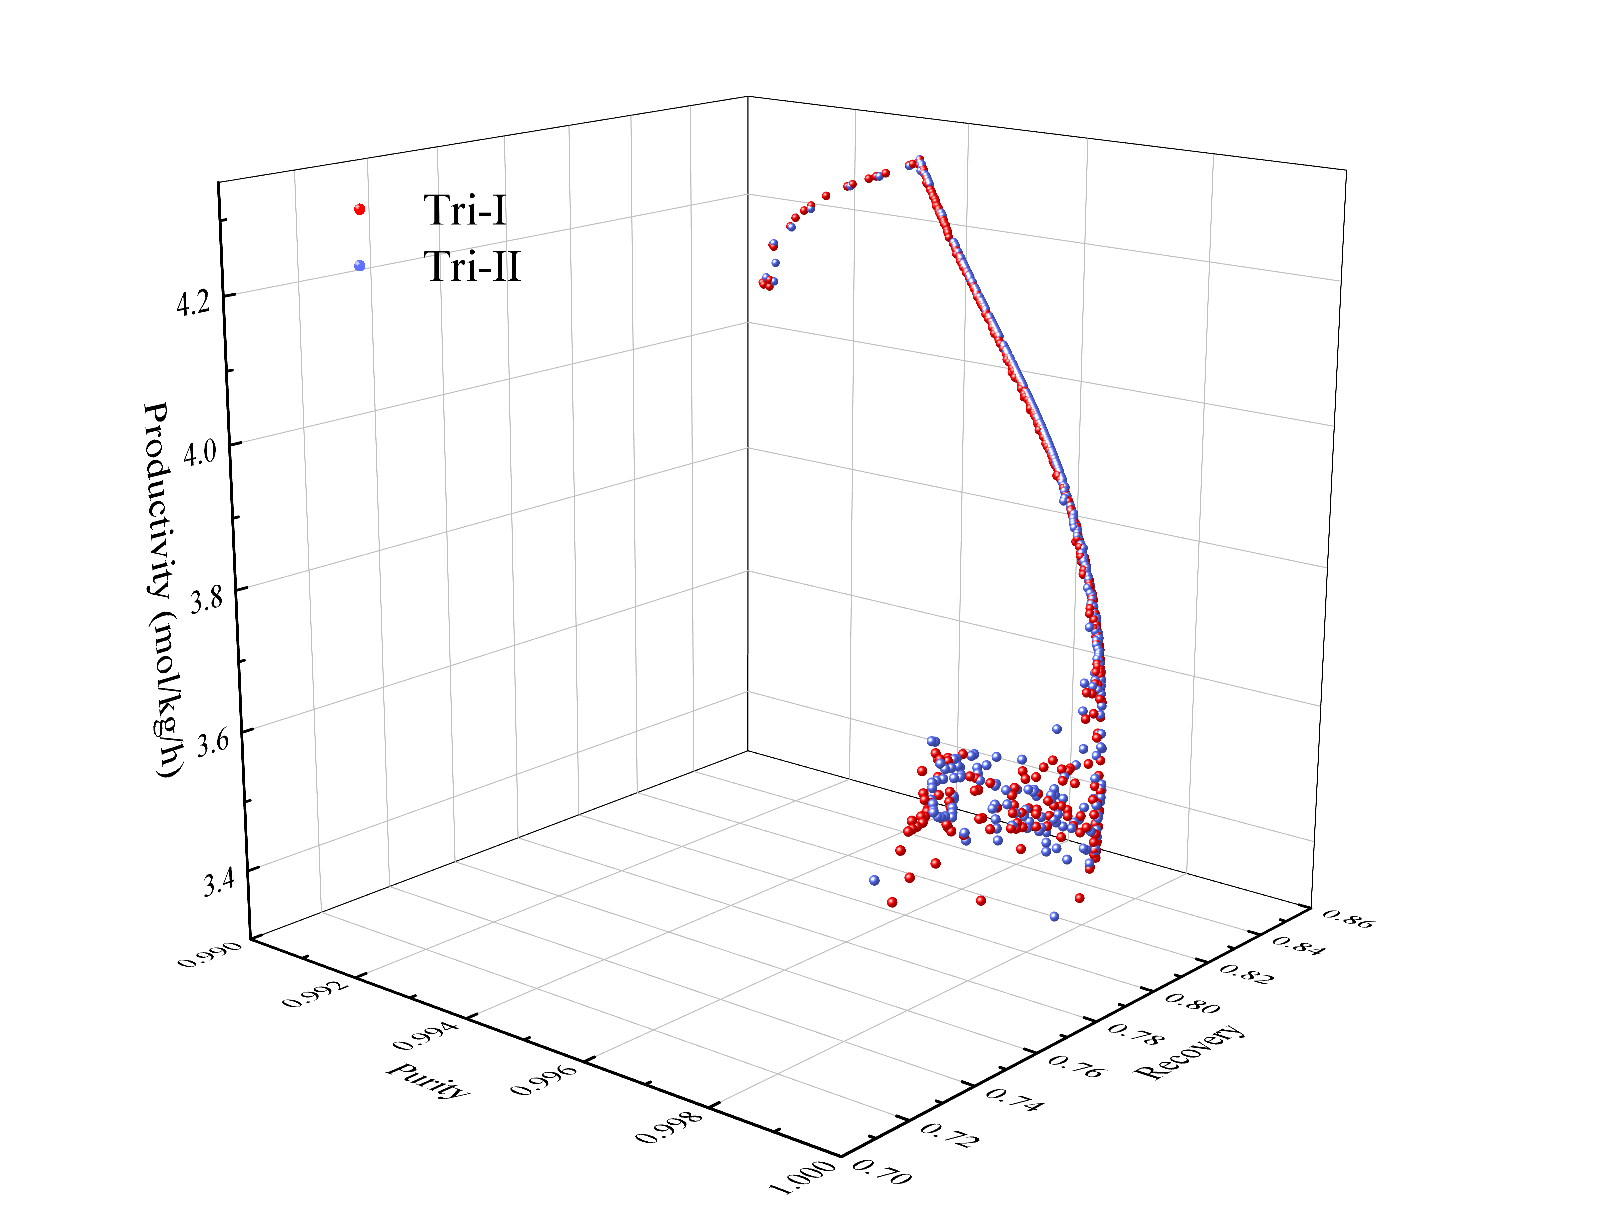
\includegraphics[width=0.5\textwidth]{figs/Fig12.pdf}
	\caption{3D Pareto-Optimal Front of Tri-objective optimization}
	\label{FIG:12}
\end{figure}
The same optimization algorithm as the previous part is used to optimize the above problem, Tri-\uppercase\expandafter{\romannumeral1} using NSGA-\uppercase\expandafter{\romannumeral2} and Tri-\uppercase\expandafter{\romannumeral2} with hybrid weight-based function. With consideration of the complexity of the problem, a larger population size and paretofraction with an order of magnitude lower tolerance are utilized to obtain more comprehensive and accurate optimization results. In order to obtain a dense solution set, we use 350 points on the Pareto front. The results of both methods are displayed in \cref{FIG:12}.

As depicted in  \cref{FIG:11} and  \cref{FIG:12}, the results obtained from the two methods are almost identical. Most points are distributed on a curve in three-dimensional space, because of the direct correlation between recovery and productivity, as shown in Eq.(4) \& Eq.(5). The accuracy of the ANN2-based surrogated model and optimization algorithm has been verified in the previous article. Otherwise, there are too many points (add up to 700) on the Pareto-Optimal sets of tri-objective optimization, so it is difficult to optimize one by one with detailed models due to huge computational consumption. Therefore, the relationship between the variables in the tri-objective optimization problem showing in Fig.S6 and Fig.S7 is used to verify the feasibility of the optimization results. Hence, the solutions provide a series of feasible operating conditions and not compromise the overall performance of the PSA process.
\begin{table}[]
	\centering
	\caption{Performance of Optimization processes}
	\begin{tabular}{lllll}
		\toprule
		& \multicolumn{2}{l}{\begin{tabular}[c]{@{}l@{}}Dual-objective   \\ optimization\end{tabular}} & \multicolumn{2}{l}{\begin{tabular}[c]{@{}l@{}}Tri-objective   \\ optimization\end{tabular}} \\
		\midrule
		& Dual-\uppercase\expandafter{\romannumeral1}                  & Dual-\uppercase\expandafter{\romannumeral2}                  & Tri-\uppercase\expandafter{\romannumeral1}                   & Tri-\uppercase\expandafter{\romannumeral2}                  \\
		Time   Consumed (S)           & 78.40                   & 32.07                   & 196.60                  & 176.13                 \\
		Total   Function Count        & 25701                   & 13222                   & 1272001                 & 1024276                \\
		Number   of Optimal Solutions & \multicolumn{2}{l}{20}                            & \multicolumn{2}{l}{350}           \\
		\bottomrule              
	\end{tabular}
\label{TABLE:8}
\end{table}
The performance indicator of all optimization processes, including time-consuming, the number of calculated equations and the number of optimal solutions, are demonstrated in \cref{TABLE:8}. The method that combines with the hybrid function uses less time than that without the hybrid function. Moreover, compared with the tens of hours consumption of the optimization based detailed models, this work consumes much less time and performs millions of function calculations at the same time. Otherwise, multi-objective optimization of ANN-based models, using genetic algorithms, provides a series of feasible process conditions, rather than an optimal advantage, and different size solution sets could be obtained by changing the parameters of NSGA-\uppercase\expandafter{\romannumeral2}.

\section{Conclusion}
This work aims to achieve multi-objective optimization using ANN-based surrogate models of pressure swing adsorption (PSA) process for hydrogen (H2)  production. A 4-bed-8-step PSA process has been investigated to produce high-purity H2 from steam methane reforming (SMR) gas mixture, which contains 76\% H2, 20\% CO2, 3.5\% CH4 and 0.5\% CO. The Detailed models of this unit consist of a series of partial differential and algebraic equations (PDAEs) and have been built in Aspen Adsorption software based on experimentally measured isotherms. 

Two different artificial neural networks have been well trained by a dataset of 100 samples obtained from the computationally expensive Detailed models based on the Latin hypercube sampling (LHS) strategy and serve as the input-output relationships to the optimize work. The ANN1 has five inputs (Xi: [PAD, t’, FAD, LAC,P/F]) and two outputs (Yi: [Purity, Recovery]), while the ANN2 has the same inputs but an additional output, Productivity. The mean square errors (MSE) and regression R values of these ANNs indicate that the performance of PSA process could be predicted with extremely high accuracy, so ANNs are feasible and suitable for the multi-objective optimization. 

Two typical multi-objective optimization problems are performed, and two different algorithms are applied to find the Pareto-Optimal solutions. The goal of Dual-objective optimization is to maximize purity and recovery with different weight and obtain Pareto-optimal Front of objective functions. The Dual-\uppercase\expandafter{\romannumeral2} method is more efficient, because the solutions obtained are slightly better than Dual-\uppercase\expandafter{\romannumeral1} and the time and total function count are reduced by half. The validation based on the simulation results of Detailed models and further analysis evidence that the non-dominated sets calculated by both optimization algorithms are accurate and feasible. The study of behaviors with PSA process have analyzed the optimal solutions and validated the performance. Two tri-objective (purity, recovery and productivity) optimizations have been complied and no significant difference between the two groups was evident. A series of feasible operating conditions is provided by the Pareto-Optimal sets. The results of all the optimizations is in line with the trend of PSA process and is validated by the outputs of Detailed models. Furthermore, the Pareto-Optimal solutions reflect the correlation between the decision variables and the optimal process conditions while provide an operated region while not compromising the overall performance of the PSA process. 
Taken together, these results suggest that artificial neural networks trained based on the samples generated by LHS Strategy and calculated using detail PSA models can approximate the performance of the PSA process with high accuracy and can be applied to the optimization as surrogate models. The multi-objective optimization using NSGA-\uppercase\expandafter{\romannumeral2} of ANN-based surrogate models can obtain a set of Pareto optimal solutions with a much less computational effort and provide a reliable reference for operational improvement.
\section{Acknowledgments}
This research is financially supported by the renewable energy and hydrogen projects in national key R \& D plan of China (2019YFB1505000).


	\bibliography{refs}

\end{document}
\endinput

